\documentclass[12pt,a4j,oneside,titlepage,fleqn]{jsbook}
%
%% パッケージ
\usepackage[dvipdfmx]{hyperref}
\usepackage{pxjahyper}
\usepackage{geometry}
\usepackage{amsmath}
\usepackage{amssymb}
\usepackage{txfonts}
\usepackage{bm}
\usepackage{titlesec}
\usepackage[dvipdfmx]{graphicx}
\usepackage{booktabs}
%
%% 設定
\geometry{top=20truemm,bottom=15truemm,left=25truemm,right=10truemm}
\setlength{\fullwidth}{175truemm}
\linespread{0.97}  % 1 ページ 40 行
\pagestyle{plain}
\setcounter{secnumdepth}{3}
\setcounter{tocdepth}{3}
\renewcommand{\prechaptername}{}
\renewcommand{\postchaptername}{.}
\renewcommand{\thesection}{\thechapter$\cdot$\arabic{section}}
\renewcommand{\thesubsection}{\thesection$\cdot$\arabic{subsection}}
\renewcommand{\thesubsubsection}{\thesubsection$\cdot$\arabic{subsubsection}}
\titleformat{\chapter}{\centering\sffamily\gtfamily\Large}{\prechaptername\thechapter\postchaptername}{1zw}{}
\titleformat{\section}{\sffamily\gtfamily\large}{\thesection}{1zw}{}
\titleformat{\subsection}{\sffamily\gtfamily\normalsize}{\thesubsection}{1zw}{}
\titleformat{\subsubsection}{\sffamily\gtfamily\normalsize}{\thesubsubsection}{1zw}{}
\titlespacing{\chapter}{0pt}{0pt}{\baselineskip}
\titlespacing{\section}{1zw}{\baselineskip}{0pt}
\titlespacing{\subsection}{1zw}{\baselineskip}{0pt}
\titlespacing{\subsubsection}{1zw}{\baselineskip}{0pt}
\renewcommand{\figurename}{Fig.~}
\renewcommand{\tablename}{Table~}
\setlength{\mathindent}{2em}
\setlength{\jot}{\baselineskip}
%
%% 表紙
\renewcommand{\maketitle}{
\begin{titlepage}
 \setcounter{page}{0}
 \begin{center}
  \vspace*{8\baselineskip}
  {○○○○年度卒業論文} \\[2\baselineskip]
  {\Large へたれテンプレート} \\[9\baselineskip]
  {○○○○年○月} \\[2\baselineskip]
  {東京理科大学理工学部機械工学科} \\[\baselineskip]
  {○○研究室} \\[3\baselineskip]
  {75*****  機械 工作}
 \end{center}
\end{titlepage}
}
%
%%%%%%%%%%%%%%%%%%%%%%%%%%%%%%%%%%%%%%%%
%
\begin{document}
%
%% 設定
\setlength{\abovedisplayskip}{\baselineskip}
\setlength{\belowdisplayskip}{\baselineskip}
%
%% 前付け
\frontmatter
\maketitle
\tableofcontents
%
%% 本文
\mainmatter
\chapter{緒言}
\section{へたれテンプレートとは?}
へたれテンプレートとは,初心者が熟練者に成長する過程でぐちゃぐちゃに改変される土台となるテンプレートです.
へたれテンプレートがどれだけぐちゃぐちゃに改変されたかを見ると,あなたがどれだけ \LaTeX に習熟したかがわかります.

\chapter{アイソジオメトリック解析手法}

\section{非一様有理Bスプライン(Non-Uniform Rational B-Spline, NURBS)}
非一様有理Bスプライン(Non-Uniform Rational B-Spline, NURBS)は,エンジニアリングデザインの中で最も広く使用される幾何学表現である.
コントロールポイントと重みを適切に設定することで,円弧等の曲線や曲面を厳密に表現できるという特徴があり,CADの形状表現にも用いられている.
NURBSはBスプライン(B-Spline)に重みを導入することで構成されており,Bスプラインは,コントロールポイントとノットベクトル,次数によって構成される.

\subsection{ノットベクトル}
Bスプラインのパラメータ空間は,パッチと呼ばれる範囲内での小領域に対してローカルに定義されるものであり,図~\ref{fig:parameter space}のように
パラメータ空間は物理空間の写像となっている.

\begin{figure}[htbp]
  \centering
  \includegraphics[keepaspectratio, scale = 1.2]
  {fig/物理空間とパラメータ空間.ai}
  \caption{B-Spline Physical space and Parametric space}
  \label{fig:parameter space}
\end{figure}

ノットベクトル(Knot vector)とは,区分的に構成されるBスプラインをつなぐ役割を持つパラメータ空間座標の座標の並びを示す単調増加のベクトルであり,パラメータ空間の
座標値$\xi, \eta$を用いて$\boldsymbol{\Xi} = \{\xi_0, \xi_1, \xi_2, \dots, \xi_{n+p}\}, \boldsymbol{H} = \{\eta_0, \eta_1, \eta_2, \dots, \eta_{m+q}\}$
と書かれる.ここで,$n, m$はBスプラインを構成するコントロールポイントの数,$p,q$は基底関数の次数である.
コントロールポイント(Control point)は物理空間上の座標であり,各軸方向のコントロールポイント数がパラメータ空間での各軸方向の基底関数の個数となる.
ノットベクトルは$n + p + 1$個の成分(ノット)によって構成される.

パラメータ空間で複数のノットを同じ値にすると,これらは重複ノットと呼ばれ,そのノットの数を重複度と呼ぶ.
IGA解析では一般に一様オープンノットベクトルと呼ばれる,最小と最大の値のノットを$p + 1$回重複させ,
他のノットを等間隔に設定したノットベクトルを用いる.
これによってBスプライン曲線の端点を表現でき,パラメータ空間上で要素を等分割することができる.
また,パラメータ空間は,物理空間の写像であるため,$\xi, \eta$の範囲は自由に設定することができるが,
プログラムの関係上,0から1までに設定するのが一般的である.

\subsection{Bスプライン基底関数}
Bスプライン基底関数はノット$\xi$を用いて以下のように表される.$p = 0$のとき

\begin{equation}
  N_{i,0}(\xi)= \left \{
  \begin{array}{l}
    1    \ \qquad $if$\  \xi_{i} \leq \xi < \xi_{i + 1} \\
    0    \ \qquad $otherwise$
  \end{array}
  \right.
  \label{eq:basis func 0}
\end{equation}

\noindent
$p = 1,2,3,\dots$のとき

\begin{equation}
  N_{i,p}(\xi)=
  \frac{\xi-\xi_i}{\xi_{i+p}-\xi_i}N_{i,p-1}(\xi)
  +\frac{\xi_{i+p+1}-\xi}{\xi_{i+p+1}-\xi_{i+1}}N_{i+1,p-1}(\xi)
  \label{eq:basis func 1}
\end{equation}

\noindent
ここで,$N_{i,p}$は次数$p$の$i$番目のBスプライン基底関数を表している.
Bスプライン基底関数には以下のような性質がある.

\begin{enumerate}
  \item 単位分割(Partition of Unity)の性質を有する.$\forall \xi$,
    \begin{equation}
      \sum_{i = 0}^{n - 1} N_{i, p}(\xi) = 1
    \end{equation}
  \item それぞれの基底関数は負の値にならない.$\forall \xi$,
    \begin{equation}
      N_{i,p}(\xi) \geq 0
    \end{equation}
  \item それぞれの$p$次の基底関数は要素境界(ノット境界)をまたいで$C^{p-1}$の連続性を持つ.
  \item ノットの重複度が$k$であるとき,そのノット上で基底関数は$C^{p-k}$連続となる.
  \item 次数$p$のBスプライン基底関数のサポートは常に$p+1$のノット間隔で行われる.
\end{enumerate}

例として,一様オープンノットベクトル$\boldsymbol{\Xi}=\{0,0,0,0.25,0.5,0.75,1,1,1, 1, 1\}$に対する
2次のBスプライン基底関数の分布を図~\ref{fig:basis func}に示す.

\begin{figure}[htbp]
  \centering
  \includegraphics[keepaspectratio, scale = 1.1]
  {fig/basis_func.ai}
  \caption{B-Spline basis function}
  \label{fig:basis func}
\end{figure}

\newpage

また,Bスプライン基底関数の導関数はノットベクトルと基底関数の次数を用いて以下のように表される.

\begin{equation}
  \label{eq:d of B-spline shape func}
  \frac{d}{d\xi}N_{i,p}(\xi) = \frac{p}{\xi_{i+p} - \xi_i}N_{i,p-1}(\xi) - \frac{p}{\xi_{i+p+1} - \xi_{i+1}}N_{i+1,p-1}(\xi)
\end{equation}

\subsection{Bスプライン曲線}
Bスプライン曲線は物理空間上の座標であるコントロールポイントを用いて線形結合で表される.
$n$個のコントロールポイント$\boldsymbol{B}_i(i = 0, 1, \dots, n-1)$,Bスプライン基底関数$N_{i, p}(i = 0, 1, \dots, n-1)$,
次数$p$,ノットベクトル$\boldsymbol{\Xi} = \{\xi_0, \xi_1, \dots, \xi_{n+p}\}$とすると,
Bスプライン曲線$\boldsymbol{C}(\xi)$は以下のように表される.

\begin{equation}
  \boldsymbol{C}(\xi)=\sum_{i=0}^{n-1} N_{i,p}(\xi)\boldsymbol{B}_i
\end{equation}

例として,一様オープンノットベクトル$\boldsymbol{\Xi}=\{0,0,0,0.25,0.5,0.75,1,1,1\}$,
コントロールポイント$\boldsymbol{B} = \{(1,2),(2,1),(3,1),(3,3),(5,3),(2,5)\}^T$に対する
2次のBスプライン曲線を図~\ref{fig:b-spline curve}に示す.

\begin{figure}[htbp]
  \centering
  \includegraphics[keepaspectratio, scale = 1.0]
  {fig/png/03.png}
  \caption{B-Spline curve and control points}
  \label{fig:b-spline curve}
\end{figure}

\newpage

\subsection{NURBS基底関数・NURBS曲線}
NURBS基底関数はBスプライン基底関数に重み(Weight)を導入した関数であり,有理式(分数式)で表現される.
NURBS曲線は,形状を制御するための要素として各コントロールポイントに対してスカラーの重みを設定し,
Bスプライン曲線を中心投影によって通常座標空間上に射影することで得られる.
$n$個のコントロールポイント$\boldsymbol{B}_i(i = 0, 1, \dots, n-1)$,重み$w_i(i = 0, 1, \dots, n-1)$,次数$p$,
Bスプライン基底関数$N_{i,p}$とすると,NURBS基底関数$R^p_i(\xi)$とNURBS曲線$\boldsymbol{C}(\xi)$は以下のように表される.

\begin{align}
  \label{eq:weight func}
  W(\xi) &= \sum_{\hat{i}=0}^{n-1}N_{\hat{i},p}(\xi)w_{\hat{i}}\\
  R^{p}_{i}(\xi)&=\frac{N_{i,p}(\xi)w_i}{W(\xi)}=\frac{N_{i,p}(\xi)w_i}{\sum_{\hat{i}=0}^{n-1}N_{\hat{i},p}(\xi)w_{\hat{i}}}\\
  \boldsymbol{C}(\xi)&=\sum_{i=0}^{n-1}R^{p}_{i}(\xi)\boldsymbol{B}_i
\end{align}

また,基底関数の次数$p$とすると
NURBS基底関数の導関数は式~(\ref{eq:d of B-spline shape func})と式~(\ref{eq:weight func})を用いて以下のように表される.

\begin{align}
  \label{eq:d of NURBS shape func}
  \frac{d}{d\xi} R^p_i (\xi) &= w_i \frac{W(\xi)N_{i,p}' - W'(\xi)N_{i,p}(\xi)}{(W(\xi))^2} \\
  W'(\xi) &= \sum^{n - 1}_{\hat{i} = 0} N'_{\hat{i},p}(\xi)w_{\hat{i}}\\
  N'_{i,p}(\xi) &\equiv \frac{d}{d\xi}N_{i,p}
\end{align}


重みは基底関数が2次の場合,図~\ref{fig:weight}に示すようなコントロールポイント
$\boldsymbol{B_1},\boldsymbol{B_2},\boldsymbol{B_3}$と重み$w_1,w_2,w_3$,
角度$\theta$を考えると,以下のように設定することで円弧を表現できる.

\begin{align}
  w_1 &= w_3 = 1\\
  w_2 &= \cos{\frac{\theta}{2}}
\end{align}

\begin{figure}[htbp]
  \centering
  \includegraphics[keepaspectratio, scale = 1.7]
  {fig/weight.ai}
  \caption{How to set weights in NURBS}
  \label{fig:weight}
\end{figure}

\newpage

Bスプライン曲線とNURBS曲線を比較した図を図~\ref{fig:compare nurbs}に示す.
コントロールポイント数や次数に依らず,適切に重みを設定したNURBS曲線は円弧と厳密に一致する.

\begin{figure}[htbp]
  \centering
  \includegraphics[keepaspectratio, scale = 0.9]
  {fig/compare_nurbs.ai}
  \caption{A comparison of B-Spline curve and NURBS curve}
  \label{fig:compare nurbs}
\end{figure}

\noindent
このNURBS基底関数を用いることにより,円錐曲線や二次曲線の正確な描写が可能となり,
重みを制御することで幾何形状の微調節も可能となる.

\subsection{NURBS曲面}
NURBS曲面は$\xi$方向の次数$p$,$\eta$方向の次数$q$,
コントロールネット$\boldsymbol{B}_{i,j}$,
重み$w_{i,j} (i=0, 1, \dots, n-1,  j=0,1, \dots, m-1)$とすると,
NURBS基底関数$R^{p,q}_{i,j}(\xi, \eta)$とNURBS曲面$\boldsymbol{S}(\xi, \eta)$は以下のように表される.

\begin{align}
  \label{NURBS basis function}
  R^{p,q}_{i,j}(\xi, \eta)&=\frac{N_{i,p}(\xi)M_{j,q}(\eta)w_{i,j}}{\sum_{\hat{i}=0}^{n-1}\sum_{\hat{j}=0}^{m-1}N_{\hat{i},p}(\xi)M_{\hat{j},q}(\eta)w_{\hat{i},\hat{j}}}\\
  \boldsymbol{S}(\xi, \eta)&=\sum_{i=0}^{n-1}\sum_{j=0}^{m-1}R^{p,q}_{i,j}(\xi, \eta)\boldsymbol{B}_{i,j}
\end{align}

NURBS曲面の例を図~\ref{fig:nurbs surface}に示す.また,3パラメータ空間まで拡張することで図~\ref{fig:tube}に示すような複雑な曲面を有する立体形状を再現できる.

\begin{figure}[htbp]
  \centering
  \includegraphics[keepaspectratio, scale = 1.0]
  {fig/png/09.png}
  \caption{NURBS surface and control points}
  \label{fig:nurbs surface}
\end{figure}

\newpage

\begin{figure}[htbp]
  \centering
  \includegraphics[keepaspectratio, scale = 0.37]
  {fig/png/04.png}
  \caption{An example of NURBS representation of a curved tube}
  \label{fig:tube}
\end{figure}

\subsection{細分化操作}
ノットベクトルとコントロールポイントを細分化する手法として,ノットインサーション(Knot Insertion)がある.
基底関数の操作は必要ないが,ノットベクトルが挿入され,コントロールポイントが増加し,さらにその物理座標が変わるため,
ノットインサーションの操作後に基底関数の計算を行う必要がある.
また,BスプラインとNURBSでやや操作が異なるため,注意が必要である.

\subsubsection{Bスプライン細分化操作}
まず,ノットベクトル$\boldsymbol{\Xi} = \{\xi_0, \xi_1, \dots, \xi_{n+p}\}$に$m$個のノットを挿入し,
挿入後のノットベクトル$\overline{\boldsymbol{\Xi}} = \{\overline{\xi}_0, \overline{\xi}_1, \dots, \overline{\xi}_{n+m+p}\}$,
コントロールポイントの行列$\boldsymbol{A} = \{\boldsymbol{B}_0, \boldsymbol{B}_1, \dots, \boldsymbol{B}_{n-1}\}^T$とすると,
ノット挿入後のコントロールポイントの行列
$\overline{\boldsymbol{A}} = \{\overline{\boldsymbol{B}}_0, \overline{\boldsymbol{B}}_1, \dots, \overline{\boldsymbol{B}}_{n+m-1}\}^T$
は以下のように表される.

\begin{equation}
  \overline{\boldsymbol{A}} = \boldsymbol{T}^p\boldsymbol{A}
  \label{eq:KI}
\end{equation}

\noindent
ここで,$\boldsymbol{T}^p$は$p = 0$のとき

\begin{equation}
  T^0_{i,j} = \left \{
  \begin{array}{l}
    1    \ \qquad $if$\  \xi_{j} \leq \overline{\xi}_i < \xi_{j + 1} \\
    0    \ \qquad $otherwise$
  \end{array}
  \right.
  \label{eq:T_0}
\end{equation}

\noindent
$p = 1,2,3,\dots$のとき

\begin{equation}
  T^p_{i,j} = \frac{\overline{\xi}_{i+p-1} - \xi_j}{\xi_{j+p-1} - \xi_j}T^{p-1}_{i,j} 
  + \frac{\xi_{j+p} - \overline{\xi}_{i+p-1}}{\xi_{j+p} - \xi_{j + 1}}T^{p-1}_{i,j+1}
  \label{eq:T_1}
\end{equation}

\noindent
以上の操作から得られたノット挿入後のノットベクトル$\overline{\boldsymbol{\Xi}}$,コントロールポイントの行列$\overline{\boldsymbol{A}}$
を用いて基底関数の計算を行うことで細分化することができる.

\subsubsection{NURBS細分化操作}
NURBSのノットインサーションでは,Bスプラインの$n$個のコントロールポイントに重みの成分を加えた行列を考え,
二次元では$\boldsymbol{B}_i = \{x_i, y_i, w_i\}(i=0,1,\dots,n-1)$をコントロールポイント座標として考える.
Bスプラインでのノットインサーションと同様に式~(\ref{eq:T_0})と式~(\ref{eq:T_1})から$\boldsymbol{T}^p$を求めた後,
式~(\ref{eq:KI})の操作を行う前に$\boldsymbol{B}_i = \{x_i\times w_i, y_i\times w_i, w_i\}(i=0,1,\dots,n-1)$と置き換えて
$\overline{\boldsymbol{A}}$を求め,さらにその成分である$\overline{\boldsymbol{B}}_j\{x_j, y_j, w_j\}(j=0,1,\dots,n+m-1)$
に対して$\overline{\boldsymbol{B}}_j\{\frac{x_j}{w_j}, \frac{y_j}{w_j}, w_j\}(j=0,1,\dots,n+m-1)$と置き換える操作を
行った後の$\overline{\boldsymbol{A}}$が細分化操作後のコントロールポイントと重みの行列となる.

NURBSのノットインサーションを行った例を図~\ref{fig:KI}に示す.

\begin{figure}[htbp]
  \centering
  \includegraphics[keepaspectratio, scale = 0.8]
  {fig/KI.ai}
  \caption{An example of NURBS Knot Insertion}
  \label{fig:KI}
\end{figure}

\subsection{高次化操作}
基底関数の次数を上げることは,式~(\ref{eq:basis func 0})と式~(\ref{eq:basis func 1})より容易であるが,
単純に次数を上げるとコントロールポイントと基底関数の線形結合で表される曲線の形状が,
次数を上げる前の曲線から変化してしまう.
形状を変えずに次数を上げ,ノットベクトルとコントロールポイントを適切に設定する高次化手法として,
オーダーエレベーション(Order Elevation)がある.
ノットインサーションと同様に基底関数を計算する前のノットベクトルとコントロールポイントに対する操作であるため,
基底関数を計算する必要はないが,非常に複雑な手順を踏む必要がある.
さらに,ノットインサーションと同様にNURBSではBスプラインと同様の操作に加えて,重みに関する処理を行う必要がある.

\subsubsection{ノット除去操作}
まず,オーダーエレベーションで必要となるノット除去操作を示す.
基本的にはノットインサーションの逆の手順を辿ることで求めることができるが,
正則ではない行列の疑似逆行列を求める過程がある.
Bスプラインのノット除去操作について考えると,
除去前のノットベクトル$\overline{\boldsymbol{\Xi}} = \{\overline{\xi}_0, \overline{\xi}_1, \dots, \overline{\xi}_{n+m+p}\}$
から$m$個のノットを除去したノットベクトル$\boldsymbol{\Xi} = \{\xi_0, \xi_1, \dots, \xi_{n+p}\}$,
ノット除去前のコントロールポイントの行列
$\overline{\boldsymbol{A}} = \{\overline{\boldsymbol{B}}_0, \overline{\boldsymbol{B}}_1, \dots, \overline{\boldsymbol{B}}_{n+m-1}\}^T$,
ノット除去後のコントロールポイントの行列$\boldsymbol{A} = \{\boldsymbol{B}_0, \boldsymbol{B}_1, \dots, \boldsymbol{B}_{n-1}\}^T$とすると,
求めたい$\boldsymbol{A}$は式~(\ref{eq:KI})と同じ式で求めることができ,$\boldsymbol{T}^p$は式~(\ref{eq:T_0})と式~(\ref{eq:T_1})から求めることができる.
$\boldsymbol{T}^p$の疑似逆行列${\boldsymbol{T}^p}^{+}$とすると,以下のように表される.

\begin{align}
  \boldsymbol{A} &= {\boldsymbol{T}^p}^{+} \overline{\boldsymbol{A}}\\
  {\boldsymbol{T}^p}^{+} &= ({\boldsymbol{T}^p}^T \boldsymbol{T}^p)^{-1} {\boldsymbol{T}^p}^T
\end{align}

\noindent
この操作を行うことで,曲線の形状を変化させることなくノットベクトルから任意のノットを取り除いたノットベクトルとコントロールポイントが得られる.

\subsubsection{Bスプライン高次化操作}
Bスプラインにおけるオーダーエレベーションの基本的な手順を以下に示す.

次数$p$とすると,
$\rm(\hspace{.18em}i\hspace{.18em})$まず,ノットベクトルの端点以外の値を重複度が$p$となるまでノットインサーションする.
ノットインサーションではBスプライン曲線形状は変化しないため,この操作により,ノットベクトルの端点以外の値で連続性が$C^0$連続となり,
Bスプライン曲線を最小のベジェ曲線(Bézier Curve)に分割することができる.
ここでベジェ曲線とは,$p+1$個のコントロールポイントから得られる$p$次曲線である.
$\rm(\hspace{.08em}ii\hspace{.08em})$次に,各ベジェ曲線で次数を上げる以下の操作を行う.
次数$p$,次数を$1$次上げた操作後の次数$\hat{p} (=p+1)$,
$p$個のコントロールポイント$\boldsymbol{B}$,操作後の$\hat{p}$個のコントロールポイント$\hat{\boldsymbol{B}}$,
$\alpha_i(i=0,1,\dots,\hat{p})$とする.

\begin{align}
  \alpha_i &= \frac{i}{\hat{p}} \\
  \hat{\boldsymbol{B}}_i &= \left \{
    \begin{array}{l}
      (1 - \alpha_i)\boldsymbol{B}_i \ \qquad \ \qquad $if$\ i = 0\\
      (1 - \alpha_i)\boldsymbol{B}_i + \alpha_i \boldsymbol{B}_{i-1} \ \ \   $otherwise$
    \end{array}
    \right.
\end{align}

\noindent
この操作を上げる次数の階数$k$だけ繰り返す.
$\rm(i\hspace{-.08em}i\hspace{-.08em}i)$その後,ノットベクトルの重複度を端点を含む全てのノットで$k$階上げる.
$\rm(i\hspace{-.08em}v\hspace{-.06em})$初めに$\rm(\hspace{.18em}i\hspace{.18em})$で挿入したノットを除去する.
以上の操作を行った後のコントロールポイントとノットベクトル,次数がそれぞれ高次化操作後の値となる.

\newpage

例として,次数$p = 2$,一様オープンノットベクトル$\boldsymbol{\Xi}=\{0,0,0,0.25,0.5,0.75,1,1,1\}$,
コントロールポイント$\boldsymbol{B} = \{(1,2),(2,1),(3,1),(3,3),(5,3),(2,5)\}^T$に対して,
次数を$1$次上げるオーダーエレベーションを行った場合の各手順での操作を以下に示す.
まず,$\rm(\hspace{.18em}i\hspace{.18em})$の操作後のBスプライン曲線を図~\ref{fig:OE_01}に示す.

\begin{figure}[htbp]
  \centering
  \includegraphics[keepaspectratio, scale = 0.8]
  {fig/OE_01.ai}
  \caption{B-Spline curve after step $\rm(\hspace{.18em}i\hspace{.18em})$ in Order Elevation}
  \label{fig:OE_01}
\end{figure}

\noindent
このとき,分割された最小のベジェ曲線は,図~\ref{fig:OE_01}におけるノットインサーション後の
$p+1$個のコントロールポイントで構成される各区間であり,それぞれのベジェ曲線に対して$\rm(\hspace{.08em}ii\hspace{.08em})$を行う.
$\rm(\hspace{.08em}ii\hspace{.08em})$及び$\rm(i\hspace{-.08em}i\hspace{-.08em}i)$の操作後のBスプライン曲線を図~\ref{fig:OE_02}に示す.

\begin{figure}[htbp]
  \centering
  \includegraphics[keepaspectratio, scale = 0.75]
  {fig/OE_02.ai}
  \caption{B-Spline curve after step $\rm(\hspace{.08em}ii\hspace{.08em})$ and $\rm(i\hspace{-.08em}i\hspace{-.08em}i)$ in Order Elevation}
  \label{fig:OE_02}
\end{figure}

\newpage

\noindent
$\rm(i\hspace{-.08em}v\hspace{-.06em})$の操作後のBスプライン曲線を図~\ref{fig:OE_03}に示す.

\begin{figure}[htbp]
  \centering
  \includegraphics[keepaspectratio, scale = 0.75]
  {fig/OE_03.ai}
  \caption{B-Spline curve after step $\rm(i\hspace{-.08em}v\hspace{-.06em})$ in Order Elevation}
  \label{fig:OE_03}
\end{figure}

\noindent
$\rm(i\hspace{-.08em}v\hspace{-.06em})$の操作後のコントロールポイント,ノットベクトル,次数がそれぞれ高次化操作後の値となる.

\subsubsection{NURBS高次化操作}
NURBSにおけるオーダーエレベーションの基本的な手順はBスプラインと同様であるが,
コントロールポイントに重みの成分を加えた行列を考え,
二次元では$\boldsymbol{B}_i = \{x_i, y_i, w_i\}(i=0,1,\dots,n-1)$をコントロールポイント座標として考える.
細分化操作でのNURBSへの拡張と同様に,$\rm(\hspace{.18em}i\hspace{.18em})$のノットインサーション,
$\rm(\hspace{.08em}ii\hspace{.08em})$の次数上げ,$\rm(i\hspace{-.08em}v\hspace{-.06em})$のノット除去の
前後でそれぞれコントロールポイント座標を置き換える操作を追加で行う必要がある.
各操作前の$n$個のコントロールポイント$\boldsymbol{B}_i = \{x_i, y_i, w_i\}(i=0,1,\dots,n-1)$を
$\boldsymbol{B}_i = \{x_i\times w_i, y_i\times w_i, w_i\}(i=0,1,\dots,n-1)$と置き換えて計算を行い,
各操作後に$m$個のコントロールポイント$\overline{\boldsymbol{B}}_j\{x_j, y_j, w_j\}(j=0,1,\dots,m-1)$を
$\overline{\boldsymbol{B}}_j\{\frac{x_j}{w_j}, \frac{y_j}{w_j}, w_j\}(j=0,1,\dots,m-1)$と置き換えることで,
NURBSでの高次化操作後のコントロールポイント,重み,ノットベクトル,次数が得られる.

\newpage

\section{アイソジオメトリック解析}
\subsection{NURBS基底関数による離散化解析}
\subsubsection{関数の定義}
物理空間からパラメータ空間への写像
$\boldsymbol{x}\ :\ \Omega \rightarrow \hat{\Omega}$は
以下のように定義される.

\begin{equation}
  \label{eq:difinement of u}
  \boldsymbol{x}(\xi)\equiv
  \begin{Bmatrix}
    x(\xi)\\
    y(\xi)
  \end{Bmatrix}
    =\sum_{a=1}^{e_{en}}N_a(\xi)
  \begin{Bmatrix}
    x^e_a\\y^e_a
  \end{Bmatrix}
\end{equation}

\noindent
ここで$N_a(\xi)$はNURBS基底関数,
${x^e_a,\ y^a_e}$は要素$e$を構成する
$a$番目のコントロールポイント$\boldsymbol{B}_a$の成分を表す.
パラメータ空間全体で他の関数についても同様に定義することができ,
パラメータ空間上の変位$\boldsymbol{u}\ :\ \Omega \rightarrow \hat{\Omega}$は
以下のように定義される.

\begin{equation}
  \boldsymbol{u}(\xi) \equiv \sum_{a=1}^{n_{en}}N_a(\xi)\boldsymbol{d}_a
\end{equation}

\noindent
ここで$\boldsymbol{d}_a$はコントロール変数と呼ばれる.

\subsubsection{境界値問題}
NURBSで定義された領域上の微分方程式を解く例として,
図~\ref{fig:boundary problem}に示すような二次元線形弾性体の境界値問題を考える.

\begin{figure}[htbp]
  \centering
  \includegraphics[keepaspectratio, scale = 0.6]
  {fig/境界値問題.ai}
  \caption{Concept of Boundary Value Problem}
  \label{fig:boundary problem}
\end{figure}

\newpage

\noindent
領域$\Omega$の固体が,物体力$\boldsymbol{b}$を受け,
ディレクレ境界$\Gamma_D$で変位固定$\overline{\boldsymbol{u}}$,
ノイマン境界$\Gamma_N$で外力$\overline{\boldsymbol{t}}$を受け,
弾性的に微小変形する.
変位$\boldsymbol{u}$,
ひずみ$\boldsymbol{\varepsilon}$,
応力$\boldsymbol{\sigma}$を求める.
領域$\Omega$の固体は,以下に示す平衡方程式(式~(\ref{eq:bvp_01})),変位ひずみ関係式(式~(\ref{eq:bvp_02})),
構成方程式(式~(\ref{eq:bvp_03})),境界条件(式~(\ref{eq:bvp_04}),式~(\ref{eq:bvp_05}))を満足する.

\begin{align}
  \label{eq:bvp_01}
  \boldsymbol{L}^T \boldsymbol{\sigma} + \boldsymbol{b} &= \boldsymbol{0} \ \ \ \qquad \qquad \rm{in} \quad \Omega\\
  \label{eq:bvp_02}
  \boldsymbol{\varepsilon} &= \boldsymbol{L} \boldsymbol{u} \qquad \qquad \rm{in} \quad \Omega\\
  \label{eq:bvp_03}
  \boldsymbol{\sigma} &= \boldsymbol{D} \boldsymbol{\varepsilon} \qquad \qquad \rm{in} \quad \Omega\\
  \label{eq:bvp_04}
  \boldsymbol{u} &= \overline{\boldsymbol{u}} \ \ \ \qquad \qquad \rm{on} \quad \Gamma_D\\
  \label{eq:bvp_05}
  \boldsymbol{t} &= \overline{\boldsymbol{t}} = \boldsymbol{n}^T \boldsymbol{\sigma} \qquad \rm{on} \quad \Gamma_N
\end{align}

\noindent
ここで,$\boldsymbol{u}$は変位ベクトル,$\boldsymbol{\varepsilon}$はひずみベクトル,
$\boldsymbol{\sigma}$は応力ベクトル,$\boldsymbol{b}$は物体力ベクトルであり,以下のように表される.

\begin{align}
  \boldsymbol{u} &= \left\{
  \begin{array}{c}
    u_1\\
    u_2
  \end{array}
  \right\}\\
  \boldsymbol{\varepsilon} &= \left\{
  \begin{array}{c}
    \varepsilon_{11}\\
    \varepsilon_{22}\\
    \gamma_{12}
  \end{array}
  \right\}\\
  \boldsymbol{\sigma} &= \left\{
  \begin{array}{c}
    \sigma_{11}\\
    \sigma_{22}\\
    \sigma_{12}
  \end{array}
  \right\}
\end{align}

\noindent
また,$\boldsymbol{L}$は微分作用素マトリクス,
$\boldsymbol{n}$は境界$\Gamma$に対する単位法線ベクトルであり,以下のように表される.

\begin{align}
  \label{eq:L}
  \boldsymbol{L} &= \left[
  \begin{array}{ccc}
    \cfrac{\partial}{\partial x} & 0\\
    0 & \cfrac{\partial}{\partial y}\\
    \cfrac{\partial}{\partial y} & \cfrac{\partial}{\partial x}
  \end{array}
  \right]\\
  \boldsymbol{n} &= \left[
    \begin{array}{ccc}
      n_1 & 0\\
      0 & n_2\\
      n_2 & n_1
    \end{array}
  \right]
\end{align}

\newpage

\noindent
$\boldsymbol{D}$は弾性マトリクスであり,ヤング率$E$,ポアソン比$\nu$とすると
平面応力状態と平面ひずみ状態でそれぞれ以下のように表される.
\begin{align}
  \label{eq:D1}
  \boldsymbol{D} &= \frac{E}{(1+\nu)(1-\nu)} \left[
    \begin{array}{ccc}
      1 & \nu & 0 \\
      \nu & 1 & 0 \\
      0 & 0 & \frac{1-\nu}{2} 
    \end{array}
  \right] &\rm{(Plane\ stress)}\\
  \label{eq:D2}
  \boldsymbol{D}&=\frac{E}{(1+\nu)(1-2\nu)} \left[
    \begin{array}{ccc}
      1-\nu & \nu & 0 \\
      \nu & 1-\nu & 0 \\
      0 & 0 & \frac{1-2\nu}{2} 
    \end{array}
  \right] &\rm{(Plane\ strain)}
\end{align}

\noindent
これらの式は境界値問題の強形式である.
強形式には唯一の厳密解が存在するが,
一般的に強形式の厳密解を解析的に求めることはできないため,
近似解を求めるための数値手法としてガラーキン法を用いる.

\subsubsection{弱形式の定義}
まず,式~(\ref{eq:bvp_01})~式~(\ref{eq:bvp_05})を近似的に満足する弱形式を定義する.
試行関数と重み関数を定義するために,$\Omega$上の自乗可積分関数空間を定義する.
この空間$L^2(\Omega)$を以下の式のような全ての関数$\boldsymbol{u}$の集合として定義する.

\begin{equation}
  \label{L2_u2_inf}
  \int_\Omega \boldsymbol{u}^2d\Omega<+\infty
\end{equation}

ここで,$d$は空間内の次元数とし,
多重指数$\boldsymbol{\alpha}\in\mathbb{N}^d$を考える.
$\boldsymbol{\alpha}=\{\alpha_1,2,\dots,\alpha_d\}$について
$|\boldsymbol{\alpha}|=\Sigma^d_{i=1}\alpha_i$を定義する.
また,微分演算子$D^j_i=\partial^j/\partial{x^j_i}$を用いて
$D^{\boldsymbol{\alpha}}=D^{\alpha_1}D^{\alpha_2}\dots D^{\alpha_d}$を定義する.
定式化に使用される特定の式が意味を成すためには
試行解の導関数が自乗可積分であることが必要であり,
$\boldsymbol{u}\ :\ \Omega\rightarrow\mathbb{R}$を試行解とすると,
次式を満たす必要がある.

\begin{equation}
  \label{nabra_u_inf}
  \int_\Omega \boldsymbol{\nabla} \boldsymbol{u}\cdot\boldsymbol{\nabla} \boldsymbol{u}d\Omega<+\infty
\end{equation}

\noindent
このような関数はソボレフ空間$H^1(\Omega)$内にある.
ソボレフ空間は以下の式で表される.

\begin{equation}
  \label{sovolev}
  H^1(\Omega)=\{\boldsymbol{u}\ |\ D^{\boldsymbol\alpha}\boldsymbol{u}\in L^2(\Omega),\ |\boldsymbol{\alpha}\le1\}
\end{equation}

\noindent
ここで$\mathcal{S}$で表す試行解の集合を,
自乗可積分微係数を持ち,$\boldsymbol{u}|_{\Gamma_D}=\overline{\boldsymbol{u}}$を満たす全ての関数として定義する.

\begin{equation}
  \label{S_trial_sol}
  \mathcal{S}=\{\boldsymbol{u}\ |\ \boldsymbol{u}\in H^1(\Omega),\ \boldsymbol{u}|_{\Gamma_D}=\overline{\boldsymbol{u}}\}
\end{equation}

\noindent
重み関数$\mathcal{V}$は以下の式で定義される.

\begin{equation}
  \label{V_trial_sol}
  \mathcal{V}=\{\boldsymbol{w}\ |\ \boldsymbol{w}\in H^1(\Omega),\ \boldsymbol{w}|_{\Gamma_D}=\boldsymbol{0}\}
\end{equation}

\noindent
式~(\ref{eq:bvp_01})に任意の重み関数$\boldsymbol{w}\in\mathcal{V}$を乗算し,
領域$\Omega$で積分することで,式~(\ref{eq:weak01})が得られる.

\begin{align}
  \int_\Omega \boldsymbol{w}^T (\boldsymbol{L}^T\boldsymbol{\sigma} + \boldsymbol{b}) d\Omega &= \boldsymbol{0} \nonumber \\
  -\int_\Omega \boldsymbol{w}^T (\boldsymbol{L}^T\boldsymbol{\sigma}) d\Omega &= \int_\Omega \boldsymbol{w}^T \boldsymbol{b} d\Omega\nonumber \\
  \label{eq:weak01}
  -\left[\int_\Omega \boldsymbol{w}^T\boldsymbol{L}^T\boldsymbol{\sigma} d\Omega - \int_\Omega (\boldsymbol{L}\boldsymbol{w})^T \boldsymbol{\sigma} d\Omega \right] &= \int_\Omega \boldsymbol{w}^T \boldsymbol{b} d\Omega
\end{align}

\noindent
ガウスの発散定理を適用することで式~(\ref{eq:weak02})が得られる.

\begin{align}
  \int_\Omega (\boldsymbol{L}\boldsymbol{w})^T \boldsymbol{\sigma} d\Omega - \int_\Gamma \boldsymbol{w}^T\boldsymbol{n}^T\boldsymbol{\sigma} d\Gamma &= \int_\Omega \boldsymbol{w}^T \boldsymbol{b} d\Omega \nonumber \\
  \label{eq:weak02}
  \int_\Omega (\boldsymbol{L}\boldsymbol{w})^T \boldsymbol{\sigma} d\Omega &= \int_\Omega \boldsymbol{w}^T \boldsymbol{b} d\Omega + \int_\Gamma \boldsymbol{w}^T \boldsymbol{t} d\Gamma
\end{align}

\noindent
ここで,$\boldsymbol{w}|_{\Gamma_D}=\boldsymbol{0}$となるので,式~(\ref{eq:weak02})の右辺第二項は以下のように表される.

\begin{align}
  \int_\Gamma \boldsymbol{w}^T \boldsymbol{t} d\Gamma &= \int_{\Gamma_N} \boldsymbol{w}^T \boldsymbol{t} d\Gamma_N + \int_{\Gamma_D} \boldsymbol{w}^T \boldsymbol{t} d\Gamma_D \nonumber \\
  \label{eq:weak03}
  &= \int_{\Gamma_N} \boldsymbol{w}^T \boldsymbol{t} d\Gamma_N
\end{align}

\noindent
また,式~(\ref{eq:bvp_05})も同様に任意の重み関数$\boldsymbol{w}\in\mathcal{V}$を乗算し,
領域$\Gamma$で積分することで,式~(\ref{eq:weak04})が得られる.

\begin{equation}
  \label{eq:weak04}
  \int _{\Gamma_N} \boldsymbol{w}^T (\boldsymbol{t} - \overline{\boldsymbol{t}}) d\Gamma = \boldsymbol{0}
\end{equation}

\newpage

\noindent
式~(\ref{eq:weak04})を式~(\ref{eq:weak03})に取り込むことで式~(\ref{eq:weak05})が得られる.

\begin{align}
  \int_\Omega (\boldsymbol{L}\boldsymbol{w})^T \boldsymbol{\sigma} d\Omega &= \int_\Omega \boldsymbol{w}^T \boldsymbol{b} d\Omega + \int_{\Gamma_N} \boldsymbol{w}^T \boldsymbol{t} d\Gamma - \int_{\Gamma_N} \boldsymbol{w}^T (\boldsymbol{t} - \overline{\boldsymbol{t}}) d\Gamma \nonumber \\
  \label{eq:weak05}
  \int_\Omega (\boldsymbol{L}\boldsymbol{w})^T \boldsymbol{\sigma} d\Omega &= \int_\Omega \boldsymbol{w}^T \boldsymbol{b} d\Omega + \int_{\Gamma_N} \boldsymbol{w}^T \overline{\boldsymbol{t}} d\Gamma
\end{align}

\noindent
応力の対称性($\sigma_{ij} = \sigma_{ji}$)と式~(\ref{eq:bvp_02}),式~(\ref{eq:bvp_03})を考慮すると,
結果として得られる問題の弱形式は以下のようになる.

\begin{equation}
  \label{eq:weak_form}
  \int_\Omega {\boldsymbol{\varepsilon}^{w}}^{T} \boldsymbol{D}\boldsymbol{\varepsilon} d\Omega = \int_\Omega \boldsymbol{w}^T \boldsymbol{b} d\Omega + \int_{\Gamma_N} \boldsymbol{w}^T \overline{\boldsymbol{t}} d\Gamma
\end{equation}

\noindent
ここで,$\boldsymbol{\varepsilon}^{w} = \boldsymbol{L}\boldsymbol{w}$である.
$\boldsymbol{a}(\boldsymbol{w},\ \boldsymbol{u})$,$\boldsymbol{L}(\boldsymbol{w})$をそれぞれ以下のように定義する.

\begin{align}
  \boldsymbol{a}(\boldsymbol{w},\ \boldsymbol{u}) &= \int_\Omega \boldsymbol{\varepsilon}^{wT} \boldsymbol{D}\boldsymbol{\varepsilon} d\Omega\\
  \boldsymbol{L}(\boldsymbol{w}) &= \int_\Omega \boldsymbol{w}^T \boldsymbol{b} d\Omega + \int_{\Gamma_N} \boldsymbol{w}^T \overline{\boldsymbol{t}} d\Gamma
\end{align}

\noindent
従って,この弱形式は以下のように書き換えることができる.

\begin{equation}
  \label{eq:weak_Galerkin}
  \boldsymbol{a}(\boldsymbol{w},\ \boldsymbol{u})=\boldsymbol{L}(\boldsymbol{w})
\end{equation}

\noindent
$\boldsymbol{a}(\cdot,\ \cdot)$は対称性を持ち,
$\boldsymbol{a}(\boldsymbol{w},\ \boldsymbol{u})=\boldsymbol{a}(\boldsymbol{u},\ \boldsymbol{w})$となる.
また,$\boldsymbol{a}(\cdot,\ \cdot)$は双線形,
$\boldsymbol{L}(\cdot)$は線形であり,全ての定数$C_1$と$C_2$に対して以下の式が成り立つ.

\begin{align}
  \boldsymbol{a} (C_1 \boldsymbol{u} + C_2 \boldsymbol{v},\ \boldsymbol{w}) &= C_1 \boldsymbol{a} (\boldsymbol{u},\ \boldsymbol{w}) + C_2 \boldsymbol{a} (\boldsymbol{v},\ \boldsymbol{w})\\
  \boldsymbol{L} (C_1 \boldsymbol{u} + C_2 \boldsymbol{v}) &= C_1 \boldsymbol{L} (\boldsymbol{u}) + C_2 \boldsymbol{L} (\boldsymbol{v})
\end{align}

\newpage

\subsubsection{ガラーキン法}
ガラ―キン法は,それぞれ$\mathcal{S}^h$と$\mathcal{V}^h$と呼ばれる
$\mathcal{S}$と$\mathcal{V}$の部分集合である有限次元近似の組み立てから成る.

\begin{align}
  \mathcal{S}^h&\subset\mathcal{S}\\
  \mathcal{V}^h&\subset\mathcal{V}
\end{align}

\noindent
式~(\ref{eq:weak_form})より,ガラーキン法の弱形式は以下のように表される.

\begin{equation}
  \label{eq:weak_form_02}
  \int_\Omega (\boldsymbol{L}\delta\boldsymbol{u}^{h})^T \boldsymbol{D}\boldsymbol{L}\boldsymbol{u}^{h} d\Omega = \int_\Omega \delta{\boldsymbol{u}^{h}}^{T} \boldsymbol{b} d\Omega + \int_{\Gamma_N} \delta{\boldsymbol{u}^{h}}^{T} \overline{\boldsymbol{t}} d\Gamma
\end{equation}

\noindent
式~(\ref{eq:weak_form_02})を式~(\ref{eq:weak_Galerkin})の形式で表したガラーキン形式は以下のように表される.

\begin{equation}
  \label{eq:Galerkin}
  \boldsymbol{a}(\delta\boldsymbol{u}^h,\ \boldsymbol{u}^h)=\boldsymbol{L}(\delta\boldsymbol{u}^h)
\end{equation}

\subsubsection{行列方程式の定義}

ガラーキン法で用いる関数空間の有限次元から関係式を導く.
解空間は任意のNURBS関数$N_A$の
線形結合で構成される.
ここで$A=1,2,\dots,n_{np}$である.
これらの関数には次式を満たす整数$n_{eq}<n_{np}$が存在すると仮定する.

\begin{equation}
  {\boldsymbol{N}_A|}_{\Gamma_D}=\boldsymbol{0}\qquad\forall A=1,2,\dots,n_{np}
\end{equation}

\noindent
定数$\boldsymbol{c}_A,A=1,2,\dots,n_{eq}$とすると,
全ての$\delta\boldsymbol{u}^h\in\mathcal{V}^h$に対して以下の式が成り立つ.

\begin{equation}
  \label{eq:delta u_vec}
  \delta\boldsymbol{u}^h=\sum^{n_{eq}}_{A=1}\boldsymbol{N}_A \boldsymbol{c}_A
\end{equation}

\noindent
$\boldsymbol{u}^h$についても同様に,$\boldsymbol{d}_A,A=1,2,\dots,n_{eq}$とすると,以下の式が成り立つ.

\begin{equation}
  \label{eq:u_vec}
  \boldsymbol{u}^h=\sum^{n_{eq}}_{A=1}\boldsymbol{N}_A \boldsymbol{d}_A
\end{equation}

\newpage

\noindent
式~(\ref{eq:Galerkin})に式~(\ref{eq:delta u_vec})と式~(\ref{eq:u_vec})を代入すると以下の式が得られる.

\begin{align}
  \boldsymbol{a} \left(
    \sum^{n_{eq}}_{A=1}\boldsymbol{N}_A\boldsymbol{c}_A,\ \sum^{n_{eq}}_{B=1}\boldsymbol{N}_B\boldsymbol{d}_B
  \right) &=
  \boldsymbol{L} \left(
    \sum^{n_{eq}}_{A=1}\boldsymbol{N}_A\boldsymbol{c}_A
  \right) \nonumber \\
  \sum^{n_{eq}}_{A=1}\boldsymbol{c}_A \left[
    \sum^{n_{eq}}_{B=1} \boldsymbol{a} (\boldsymbol{N}_A,\ \boldsymbol{N}_B\boldsymbol{d}_B) - \boldsymbol{L} (\boldsymbol{N}_A)
  \right] &= 0 \nonumber \\
  \label{eq:u temp01}
  \sum^{n_{eq}}_{A=1}\boldsymbol{c}_A \left[
    \sum^{n_{eq}}_{B=1} \boldsymbol{a} (\boldsymbol{N}_A,\ \boldsymbol{N}_B)\boldsymbol{d}_B - \boldsymbol{L} (\boldsymbol{N}_A)
  \right] &= 0
\end{align}

\noindent
式~(\ref{eq:u temp01})は任意の$\boldsymbol{c}_A$で成立するので,以下の式が成り立つ.

\begin{equation}
  \label{eq:u temp02}
  \sum^{n_{eq}}_{B=1} \boldsymbol{a} (\boldsymbol{N}_A,\ \boldsymbol{N}_B)\boldsymbol{d}_B = \boldsymbol{L} (\boldsymbol{N}_A)
\end{equation}

\noindent
ここで,以下のように定義する.

\begin{align}
  \boldsymbol{K} &= \boldsymbol{K}_{AB} = \boldsymbol{a} (\boldsymbol{N}_A, \boldsymbol{N}_B)\\
  \boldsymbol{F} &= \boldsymbol{F}_{A} = \boldsymbol{L} (\boldsymbol{N}_A)\\
  \boldsymbol{d} &= \boldsymbol{d}_B
\end{align}

\noindent
式~(\ref{eq:u temp02})は以下のような行列方程式となる.

\begin{equation}
  \label{eq:u temp03}
  \boldsymbol{K}\boldsymbol{d} = \boldsymbol{F}
\end{equation}

\noindent
ここで,$\boldsymbol{K}$は剛性マトリクス,$\boldsymbol{d}$は変位ベクトル,$\boldsymbol{F}$は外力ベクトルである.
$\boldsymbol{d}$を求めるため,式~(\ref{eq:u temp03})より以下の式を得る.

\begin{equation}
  \boldsymbol{d} = \boldsymbol{K}^{-1}\boldsymbol{F}
\end{equation}

\newpage

\subsubsection{二次元線形弾性問題}
二次元線形弾性問題においてひずみベクトルを以下のように定義する.

\begin{equation}
  \label{eq:epsilon}
  \boldsymbol{\varepsilon}=
    \begin{Bmatrix}
      \varepsilon_{11}\\
      \varepsilon_{22}\\
      \gamma_{12}
    \end{Bmatrix}=
    \begin{Bmatrix}
      \cfrac{\partial u_1}{\partial x}\\
      \cfrac{\partial u_2}{\partial y}\\
      \cfrac{\partial u_1}{\partial y}+\cfrac{\partial u_2}{\partial x}
    \end{Bmatrix}=
    \left[
      \begin{array}{cc}
        \cfrac{\partial}{\partial x} & 0\\
        0 & \cfrac{\partial}{\partial y}\\
        \cfrac{\partial}{\partial y} & \cfrac{\partial}{\partial x}
      \end{array}
    \right]
    \begin{Bmatrix}
      u_1\\
      u_2
    \end{Bmatrix}
\end{equation}

\noindent
式~(\ref{eq:u_vec})と式~(\ref{eq:epsilon})より,離散化されたひずみベクトルは以下のように表される.

\begin{equation}
  \boldsymbol{\varepsilon} = \boldsymbol{L}(\boldsymbol{N}\boldsymbol{d})=\boldsymbol{B}\boldsymbol{d}
\end{equation}

\noindent
ここで,$\boldsymbol{L}$は式~(\ref{eq:L})に示す微分作用素,$\boldsymbol{B}$は変位ひずみマトリクスであり,以下のように表される.

\begin{equation}
  \boldsymbol{B} = \boldsymbol{L}\boldsymbol{N} = \left[
    \begin{array}{cc}
       \cfrac{\partial N}{\partial x} & 0 \\
      0 & \cfrac{\partial N}{\partial y} \\
      \cfrac{\partial N}{\partial y} & \cfrac{\partial N}{\partial x} 
    \end{array}
  \right]
\end{equation}

\noindent
また,二次元線形弾性問題の応力ひずみ関係は構成方程式により定義され,
応力ベクトルは式~(\ref{eq:D1})と式~(\ref{eq:D2})に示す弾性マトリクス$\boldsymbol{D}$を用いて以下のように定義される.

\begin{equation}
  \boldsymbol{\sigma}=\boldsymbol{D}\boldsymbol{\varepsilon}
\end{equation}

\subsection{IGAにおける要素}
FEMでは節点座標を線分で繋ぐことで任意の形状のメッシュを作成し,
メッシュ内の領域を要素と定義するが,
IGAではコントロールポイント座標ではなく,
ノットベクトルで仕切られた区間を要素と定義される.
一方向について考えると,コントロールポイント数$n$個,
次数$p$とすると,ノットベクトルの長さは$n+p+1$となり,
一様オープンノットベクトルの場合,パッチ境界であるノットベクトルの両端でそれぞれ$p+1$の重複度とするため,
この方向の要素の数は$n-p$個となる.
従って,同じコントロールポイント数でも次数が異なる場合では要素数が変化する.

\newpage

\subsection{数値積分のための写像}
IGAでは数値積分法としてガウス・ルジャンドル積分法(Gauss-Legendre Quadrature)を用いる.
積分点数$n$,数値積分の重み$w_i$,被積分関数$f(x)$とすると,
ガウス・ルジャンドル積分法は以下のように定義される.

\begin{equation}
  \int^1_{-1} f(x)dx \approx \sum^n_{i=1}w_if(x_i)
\end{equation}

\noindent
積分点数によって適切な座標$x_i$と重み$w_i$を用いて計算を行うことで,
$2n-1$次関数までの正確な積分が可能となる.
ガウス積分は$[-1,1]$の領域で行う必要があるが,IGAでは要素によってノットの領域が異なるため,
図~\ref{fig:parent space}に示すような親要素空間を定義し,この空間でガウス・ルジャンドル積分を行う.

\begin{figure}[htbp]
  \centering
  \includegraphics[keepaspectratio, scale = 0.85]
  {fig/parent_space.ai}
  \caption{Physical space, Parametric space and Parent element space}
  \label{fig:parent space}
\end{figure}

\noindent
この親要素空間からパラメータ空間のそれぞれの要素へ変換し,
パラメータ空間から物理空間へ変換する,という流れで計算を行う.
物理空間の座標を$\boldsymbol{x}$,パラメータ空間の座標を$\boldsymbol{\xi}$,親要素空間の座標を$\tilde{\boldsymbol{\xi}}$
とし,
物理座標の要素を$\Omega^e$,パラメータ空間の要素を$\hat{\Omega}^e$,親要素空間の要素を$\tilde{\Omega}^e$とする.
図~\ref{fig:parent space}に示すようなパラメータ空間の要素$\hat{\Omega}^e$を考えると,
以下のような関係が成り立つ.

\begin{align}
  \label{eq:parent01}
  \xi &= \xi_i + (\tilde{\xi} + 1) \frac{\xi_{i+1} - \xi_i}{2}\\
  \label{eq:parent02}
  \eta &= \eta_j + (\tilde{\eta} + 1) \frac{\eta_{j+1} - \eta_j}{2}
\end{align}

\noindent
従って,親要素空間の座標$(\tilde{\xi},\ \tilde{\eta})\in \tilde{\Omega}^e$から
パラメータ空間の座標$(\xi,\ \eta)\in \hat{\Omega}^e$を求められる.
% \chapter{重合パッチ法}
\section{重合パッチ法の理論}
重合パッチ法による解析では,
全体の構造をIGAグローバルパッチで離散化し,
詳細な領域ではIGAローカルパッチで離散化し,
グローバルパッチとローカルパッチを重ね合わせて解析を行う.
図~\ref{fig:Concept S-IGA}に示すように,グローバル領域$\Omega^G$,ローカル領域$\Omega^L$,グローバル領域の境界$\Gamma^G$,
ローカル領域の境界$\Gamma^L$,グローバル領域上のローカル領域の境界$\Gamma^{GL}$とする.

\begin{figure}[htbp]
  \centering
  \includegraphics[keepaspectratio, scale = 0.7]
  {fig/重合パッチ_v2.ai}
  \caption{Concept of S-IGA}
  \label{fig:Concept S-IGA}
\end{figure}

\noindent
添え字$G,L$はそれぞれグローバル領域$\Omega^G$,ローカル領域$\Omega^L$に関する物理量量であることを示す表記である.
$\Omega^G,\Omega^L$ではそれぞれ独立の変位場$\boldsymbol{u}^G,\boldsymbol{u}^L$が定義されており,$\Omega^L$上での実際の変位は
$\Omega^G,\Omega^L$での変位を重ね合わせた和で以下のように定義される.

\begin{equation}
  \label{eq:ugul}
  \boldsymbol{u} = \left \{
    \begin{array}{l}
      \boldsymbol{u}^G  \ \ \ \quad \qquad $in$ \quad \Omega^G \cap \overline{\Omega^L}\\
      \boldsymbol{u}^G+\boldsymbol{u}^L \ \ \ \quad $in$ \quad \Omega^L
    \end{array}
  \right.
\end{equation}

\noindent
また,$\Gamma^{GL}$での変位の$C^0$連続性を保証するため以下のような条件を課す.

\begin{equation}
  \boldsymbol{u}^L = \boldsymbol{0} \ \ \ \quad $on$ \quad \Gamma^{GL}
\end{equation}

\noindent
式~(\ref{eq:ugul})を偏微分することで,ひずみは以下のように表される.

\begin{equation}
  \boldsymbol{\varepsilon} = \left \{
    \begin{array}{l}
      \boldsymbol{L}\boldsymbol{u}^G = \boldsymbol{\varepsilon}^G \ \ \ \ \ \  \qquad \qquad \qquad \qquad \qquad \quad $in$ \quad \Omega^G \cap \overline{\Omega^L}\\
      \boldsymbol{L}(\boldsymbol{u}^G+\boldsymbol{u}^L)=\boldsymbol{L}\boldsymbol{u}^G+\boldsymbol{L}\boldsymbol{u}^L=\boldsymbol{\varepsilon}^G+\boldsymbol{\varepsilon}^L \qquad $in$ \quad \Omega^L
    \end{array}
  \right.
\end{equation}

\noindent
ここで,$\boldsymbol{L}$は,式~(\ref{eq:L})で表される二次元の微分作用素である.
領域$\Omega^G$,領域$\Omega^L$において,変位場及びひずみ場は形状関数を用いて離散化され,以下のように表される.

\begin{eqnarray}
  \boldsymbol{u}^G&=\boldsymbol{N}^G\boldsymbol{d}^G\\
  \boldsymbol{u}^L&=\boldsymbol{N}^L\boldsymbol{d}^L\\
  \boldsymbol{\varepsilon}^G&=\boldsymbol{B}^G\boldsymbol{u}^G\\
  \boldsymbol{\varepsilon}^L&=\boldsymbol{B}^L\boldsymbol{u}^L
\end{eqnarray}

\noindent
ここで,$\boldsymbol{N}^G$,$\boldsymbol{N}^L$はNURBS基底関数マトリクス,
$\boldsymbol{d}^G,\boldsymbol{d}^L$はコントロールポイント変位ベクトル,
$\boldsymbol{B}^G$,$\boldsymbol{B}^L$は変位ひずみマトリクスである.
このときグローバルパッチとローカルパッチの
コントロールポイントやノットベクトルが一致する必要はない.

上記の仮定を仮想仕事の原理に代入し,離散化されたつりあい方程式を導く.
ここで,仮想変位$\delta \boldsymbol{u}$,仮想ひずみ$\delta \boldsymbol{\varepsilon}$は,変位,ひずみと同様に
グローバルパッチとローカルパッチの重ね合わせで表現され,以下のように表される.

\begin{align}
  \delta \boldsymbol{u} &= \delta \boldsymbol{u}^G + \delta \boldsymbol{u}^L\\
  \delta \boldsymbol{\varepsilon} &= \delta \boldsymbol{\varepsilon}^G + \delta \boldsymbol{\varepsilon}^L
\end{align}

\noindent
線形弾性体の場合,仮想仕事の原理は以下のように表される.

\begin{equation}
  \label{eq:VW01}
  \int_\Omega \delta \boldsymbol{\varepsilon}^T \boldsymbol{D} \boldsymbol{\varepsilon} d\Omega
  = \int_\Omega \delta \boldsymbol{u}^T \boldsymbol{b} d\Omega + \int_{\Gamma^t} \delta \boldsymbol{u}^T \boldsymbol{t} d\Gamma
\end{equation}

\noindent
ここで,$\boldsymbol{D}$は弾性マトリクス,$\boldsymbol{b}$は体積力ベクトル,
$\boldsymbol{t}$は表面力ベクトルである.
式~(\ref{eq:VW01})の左辺を$\Omega^G\cap\overline{\Omega^L}$と$\Omega^L$の二つの領域に分割すると以下のように表される.

\begin{align}
  \int_{\Omega} \delta\boldsymbol{\varepsilon}^T\boldsymbol{D}\boldsymbol{\varepsilon} d\Omega
  &=\int_{\Omega^G\cap\overline{\Omega^L}} \delta{\boldsymbol{\varepsilon}^G}^T\boldsymbol{D}\boldsymbol{\varepsilon}^G d\Omega
  +\int_{\Omega^L} \delta({\boldsymbol{\varepsilon}^G}^T+{\boldsymbol{\varepsilon}^L}^T)\boldsymbol{D}(\boldsymbol{\varepsilon}^G+\boldsymbol{\varepsilon}^L) d\Omega \nonumber \\
  &=\int_{\Omega^G} \delta{\boldsymbol{\varepsilon}^G}^T\boldsymbol{D}\boldsymbol{\varepsilon}^G d\Omega
  +\int_{\Omega^L} \delta{\boldsymbol{\varepsilon}^G}^T\boldsymbol{D}\boldsymbol{\varepsilon}^L d\Omega
  +\int_{\Omega^L} \delta{\boldsymbol{\varepsilon}^L}^T\boldsymbol{D}\boldsymbol{\varepsilon}^G d\Omega
  +\int_{\Omega^L} \delta{\boldsymbol{\varepsilon}^L}^T\boldsymbol{D}\boldsymbol{\varepsilon}^L d\Omega
\end{align}

\noindent
式~(\ref{eq:VW01})の右辺についても同様に,$\Omega^G\cap\overline{\Omega^L}$と$\Omega^L$の二つの領域に分割すると以下のように表される.

\begin{equation}
  \int_\Omega \delta\boldsymbol{u}^T\boldsymbol{b} d\Omega+\int_{\Gamma^t} \delta\boldsymbol{u}^T\boldsymbol{t} d\Gamma
  =\int_{\Omega^G} \delta{\boldsymbol{u}^G}^T\boldsymbol{b} d\Omega+\int_{\Gamma^t} \delta{\boldsymbol{u}^G}^T\boldsymbol{t} d\Gamma
  +\int_{\Omega^L} \delta{\boldsymbol{u}^L}^T\boldsymbol{b} d\Omega+\int_{\Gamma^t} \delta{\boldsymbol{u}^L}^T\boldsymbol{t} d\Gamma
\end{equation}

\noindent
仮想変位の任意性から,離散化したつりあい方程式は以下のように表される.

\begin{equation}
  \label{eq:K_array}
  \begin{bmatrix}
    \boldsymbol{K}^G & \boldsymbol{K}^{GL} \\
    \boldsymbol{K}^{LG} & \boldsymbol{K}^L
  \end{bmatrix}
  \left\{
  \begin{array}{c}
    \boldsymbol{d}^G \\
    \boldsymbol{d}^L
  \end{array}
  \right\} =
  \left\{
  \begin{array}{c}
    \boldsymbol{f}^G \\
    \boldsymbol{f}^L
  \end{array}
  \right\}
\end{equation}

\noindent
ここで,以下のような式が成り立つ.

\begin{eqnarray}
  \boldsymbol{K}^G&=\int_{\Omega^G} {\boldsymbol{B}^G}^T\boldsymbol{D}\boldsymbol{B}^Gd\Omega\\
  \boldsymbol{K}^L&=\int_{\Omega^L} {\boldsymbol{B}^L}^T\boldsymbol{D}\boldsymbol{B}^Ld\Omega\\
  \boldsymbol{K}^{GL}&=\int_{\Omega^L} {\boldsymbol{B}^G}^T\boldsymbol{D}\boldsymbol{B}^Ld\Omega\\
  \boldsymbol{K}^{LG}&=\int_{\Omega^L} {\boldsymbol{B}^L}^T\boldsymbol{D}\boldsymbol{B}^Gd\Omega\\
  \boldsymbol{f}^{G}&=\int_{\Omega^G} {\boldsymbol{N}^G}^T\boldsymbol{b}d\Omega+\int_{\Gamma^t} {\boldsymbol{N}^G}^T\boldsymbol{t}d\Gamma\\
  \boldsymbol{f}^{L}&=\int_{\Omega^L} {\boldsymbol{N}^L}^T\boldsymbol{b}d\Omega+\int_{\Gamma^t} {\boldsymbol{N}^L}^T\boldsymbol{t}d\Gamma
\end{eqnarray}

\noindent
$\boldsymbol{K}^G$,$\boldsymbol{K}^L$はそれぞれ,グローバルパッチ及びローカルパッチ上で定義される通常の剛性マトリクスである.
$\boldsymbol{K}^{GL}$,$\boldsymbol{K}^{LG}$は両パッチの連成を表すマトリクスであり,結合剛性マトリクスと呼ぶ.
$\boldsymbol{K}^{LG}$はその定義から$\boldsymbol{K}^{GL}$の転置行列となるので,
式~(\ref{eq:K_array})は以下のように書き換えることができる.

\begin{equation}
    \begin{bmatrix}
      \boldsymbol{K}^G & \boldsymbol{K}^{GL} \\
      {\boldsymbol{K}^{GL}}^T & \boldsymbol{K}^L
    \end{bmatrix}
    \left\{
    \begin{array}{c}
      \boldsymbol{d}^G \\
      \boldsymbol{d}^L
    \end{array}
    \right\} =
    \left\{
    \begin{array}{c}
      \boldsymbol{f}^G \\
      \boldsymbol{f}^L
    \end{array}
    \right\}
\end{equation}

\section{結合剛性マトリクス}
結合剛性マトリクス$\boldsymbol{K}^{GL}$の積分計算は
ローカルパッチ上の要素であるローカル要素に対して行う.
ローカル要素の物理座標での数値積分を親要素空間に変換し,
ガウス・ルジャンドル積分を用いて数値積分を行うと以下のように表される.

\begin{align}
  \boldsymbol{K}^{GL}&=\int_{\Omega^L} {\boldsymbol{B}^G}^T\boldsymbol{D}\boldsymbol{B}^Ld\Omega \nonumber \\
  &=\iint_{\Omega^L} {\boldsymbol{B}^G}^T\boldsymbol{D}\boldsymbol{B}^Ldx dy \nonumber \\
  &=\int_{-1}^1\int_{-1}^1 {\boldsymbol{B}^G}^T\boldsymbol{D}\boldsymbol{B}^L|\boldsymbol{J}|d\tilde{\xi} d\tilde{\eta} \nonumber \\
  &=\sum^m_{j=1}\sum^n_{i=1} {\boldsymbol{B}^G}^T\left(\tilde{\xi}_i^G,\tilde{\eta}_j^G\right)\boldsymbol{D}\boldsymbol{B}^L\left(\tilde{\xi}_i^L,\tilde{\eta}_j^L\right)|\boldsymbol{J}|w_iw_j
\end{align}

\noindent
ここで,$n,m,w_i,w_j$はそれぞれガウス・ルジャンドル積分での各方向の積分点数,重みである.
$|\boldsymbol{J}|$はヤコビアンの行列式であり,ヤコビアンの導出を以下に示す.

\begin{equation}
  \boldsymbol{J} = \left[
    \frac{\partial \boldsymbol{x}}{\partial \boldsymbol{\tilde{\xi}}}
  \right] =
  \left[
    \begin{array}{cc}
      \cfrac{\partial x}{\partial \tilde{\xi}} & \cfrac{\partial x}{\partial \tilde{\eta}}\\
      \cfrac{\partial y}{\partial \tilde{\xi}} & \cfrac{\partial y}{\partial \tilde{\eta}}
    \end{array}
  \right] =
  \left[
    \begin{array}{cc}
      \cfrac{\partial x(\xi,\ \eta)}{\partial R(\xi,\ \eta)} \cfrac{\partial R(\xi,\ \eta)}{\partial \xi} \cfrac{\partial \xi}{\partial \tilde{\xi}} & \cfrac{\partial x(\xi,\ \eta)}{\partial R(\xi,\ \eta)} \cfrac{\partial R(\xi,\ \eta)}{\partial \eta} \cfrac{\partial \eta}{\partial \tilde{\eta}}\\
      \cfrac{\partial y(\xi,\ \eta)}{\partial R(\xi,\ \eta)} \cfrac{\partial R(\xi,\ \eta)}{\partial \xi} \cfrac{\partial \xi}{\partial \tilde{\xi}} & \cfrac{\partial y(\xi,\ \eta)}{\partial R(\xi,\ \eta)} \cfrac{\partial R(\xi,\ \eta)}{\partial \eta} \cfrac{\partial \eta}{\partial \tilde{\eta}}
    \end{array}
  \right]
\end{equation}

\noindent
式~(\ref{eq:difinement of u})より,以下の式が得られる.

\begin{align}
  \frac{\partial x(\xi,\ \eta)}{\partial R(\xi,\ \eta)} &= \sum^{n_{en}}_{a = 1} x^e_a\\
  \frac{\partial y(\xi,\ \eta)}{\partial R(\xi,\ \eta)} &= \sum^{n_{en}}_{a = 1} y^e_a\\
  \boldsymbol{X} &\equiv \left[
    \begin{array}{c}
      \boldsymbol{x}^e\\
      \boldsymbol{y}^e
    \end{array}
  \right]^T = \left[
    \begin{array}{cccc}
      x^e_1 & x^e_2 & \cdots & x^e_{n_{en}}\\
      y^e_1 & y^e_2 & \cdots & y^e_{n_{en}}
    \end{array}
  \right]^T
\end{align}

\newpage

\noindent
式~(\ref{eq:d of NURBS shape func})を2パラメータ空間のNURBS曲面に拡張した式を考えると,以下の式が得られる.

\begin{align}
  \frac{\partial R(\xi,\ \eta)}{\partial \xi}  &= \frac{\partial}{\partial \xi}R^{p,q}_a(\xi,\ \eta)\\
  \frac{\partial R(\xi,\ \eta)}{\partial \eta} &= \frac{\partial}{\partial \eta}R^{p,q}_a(\xi,\ \eta)\\
  \boldsymbol{R}'^{a} &\equiv \left\{
    \begin{array}{c}
      \cfrac{\partial}{\partial \xi}R^{p,q}_a(\xi,\ \eta)\\
      \cfrac{\partial}{\partial \eta}R^{p,q}_a(\xi,\ \eta)
    \end{array}
  \right\}
\end{align}

\noindent
また,図~\ref{fig:parent space}に示すような座標変換を考えると式~(\ref{eq:parent01})及び式~(\ref{eq:parent02})より,
以下の式が得られる.

\begin{align}
  \frac{\partial \xi}{\partial \tilde{\xi}} &= \frac{\xi_{i+1} - \xi_i}{2}\\
  \frac{\partial \eta}{\partial \tilde{\eta}} &= \frac{\eta_{j+1} - \eta_j}{2}\\
  \boldsymbol{P}' &\equiv \left\{
    \begin{array}{c}
      \cfrac{\xi_{i+1} - \xi_i}{2}\\
      \cfrac{\eta_{j+1} - \eta_j}{2}
    \end{array}
  \right\}
\end{align}

\noindent
従って,ヤコビアンは式~(\ref{eq:JAC})のように表される.

\begin{equation}
  \label{eq:JAC}
  J_{\hat{i}\hat{j}} = \sum^{n_{en}}_{a=1} X_{a\hat{i}} R'^{a}_{\hat{j}} P'_{\hat{j}}
\end{equation}

$\boldsymbol{B}^G$の計算は,
積分点の座標値としてローカルパッチ上の親要素空間の座標$(\tilde{\xi}_i^L,\tilde{\eta}_j^L)$ではなく,
グローバルパッチ上の親要素空間の座標$(\tilde{\xi}_i^G,\tilde{\eta}_j^G)$を利用するため,
座標変換が必要となる.
ローカルパッチ上の親要素空間からグローバルパッチ上の親要素空間への
座標変換は以下の手順で行う.

\begin{enumerate}
  \item 各積分点のローカルパッチ上の親要素空間の座標$(\tilde{\xi}_i^L,\tilde{\eta}_j^L)$を
        ローカルパッチ上のパラメータ空間の座標$(\xi_i^L,\eta_j^L)$に変換する.
  \item ローカルパッチ上のパラメータ空間の座標$(\xi_i^L,\eta_j^L)$を
        ローカルパッチ上の物理空間の座標$(x,y)$に変換する.
  \item 物理空間の座標$(x,y)$を
        グローバルパッチ上のパラメータ空間の座標$(\xi_i^G,\eta_j^G)$に変換する.
  \item グローバルパッチ上のパラメータ空間の座標$(\xi_i^G,\eta_j^G)$を
        グローバルパッチ上の親要素空間の座標$(\tilde{\xi}_i^G,\tilde{\eta}_j^G)$に変換する.
\end{enumerate}

\begin{figure}[htbp]
  \centering
  \includegraphics[keepaspectratio, scale = 0.85]
  {fig/Coordinate_Transformation.ai}
  \caption{Coordinate Transformation between Global patch and Local patch}
  \label{fig:Coordinate Transformation}
\end{figure}

\noindent
図~\ref{fig:Coordinate Transformation}に示す手順で座標変換を行うが,物理空間の座標をグローバルパッチ上のパラメータ空間の座標に変換する際,
Newtoon-Raphson法を用いる.
まず,物理空間座標を$(x_i,y_j)=(X,Y)$として
以下の方程式を定義する.

\begin{equation}
  \left\{
  \begin{array}{l}
    f(\xi^G,\eta^G)=X-x(\xi^G,\eta^G)=0\\
    g(\xi^G,\eta^G)=Y-y(\xi^G,\eta^G)=0
  \end{array}
  \right.
\end{equation}

\noindent
これらを満たす$(\xi^G,\eta^G)$を反復計算で求めることを考える.
反復回数を$n$とすると,二次元のNewton-Raphson法は以下のように定義できる.

\begin{align}
  \left\{
    \begin{array}{l}
      \xi^G_{n+1}\\
      \eta^G_{n+1}
    \end{array}
  \right\}&=
  \left\{
    \begin{array}{l}
      \xi^G_{n}\\
      \eta^G_{n}
    \end{array}
  \right\}-
  {\left[
    \begin{array}{cc}
      \cfrac{\partial{f(\xi^G,\eta^G)}}{\partial{\xi^G}} & \cfrac{\partial{f(\xi^G,\eta^G)}}{\partial{\eta^G}} \\
      \cfrac{\partial{g(\xi^G,\eta^G)}}{\partial{\xi^G}} & \cfrac{\partial{g(\xi^G,\eta^G)}}{\partial{\eta^G}}
    \end{array}
  \right]}^{-1}
  \left\{
    \begin{array}{l}
      f(\xi^G_n,\eta^G_n)\\
      g(\xi^G_n,\eta^G_n)
    \end{array}
  \right\} \nonumber \\
  &=
  \left\{
    \begin{array}{l}
      \xi^G_{n}\\
      \eta^G_{n}
    \end{array}
  \right\}+
  {\left[
    \begin{array}{cc}
      \cfrac{\partial{x(\xi^G,\eta^G)}}{\partial{\xi^G}} & \cfrac{\partial{x(\xi^G,\eta^G)}}{\partial{\eta^G}} \\
      \cfrac{\partial{y(\xi^G,\eta^G)}}{\partial{\xi^G}} & \cfrac{\partial{y(\xi^G,\eta^G)}}{\partial{\eta^G}}
    \end{array}
  \right]}^{-1}
  \left\{
    \begin{array}{l}
      X-x(\xi^G_n,\eta^G_n)\\
      Y-y(\xi^G_n,\eta^G_n)
    \end{array}
  \right\}
\end{align}

\noindent
$(\xi,\eta)$の初期値$(\xi_0,\eta_0)$は
グローバルパッチ上のノットベクトルの最小値と最大値を用いて
以下のように定義した.

\begin{align}
  \xi_0&=\frac{\xi^G_{\rm{min}}+\xi^G_{\rm{max}}}{2}\\
  \eta_0&=\frac{\eta^G_{\rm{min}}+\eta^G_{\rm{max}}}{2}
\end{align}

\noindent
また,収束判定には以下の条件を用いた.

\begin{equation}
  {\left(X-x(\xi_n,\eta_n)\right)}^2+{\left(Y-y(\xi_n,\eta_n)\right)}^2<\varepsilon
\end{equation}

\noindent
本研究では$\varepsilon=1.0\times10^{-14}$として,
反復計算でグローバルパッチ上のパラメータ空間座標を算出した.
% \chapter{数値解析例}
本研究では,全ての解析問題を線形弾性問題として解析を行った.連立一次方程式の求解には
共役勾配法(Conjurate Gradient Method, CG法)を用いており,
収束判定のしきい値を相対残差で$10^{-13}$とした.

\section{3次の基底関数を用いたIGA解析}
通常のIGA解析を行い,2次と
3次の基底関数を用いた解析の誤差精度の検証を行った.

\subsection{内圧を受ける厚肉円筒の解析}
解析対象は,外径$4\ $mm,内径$2\ $mmの厚肉円筒であり,解析には二次元の$1/4$モデルを使用した.
解析問題を図~\ref{fig:internal pressure}に示す.
平面ひずみ状態を仮定し,ヤング率は$206\ $GPa,ポアソン比は$0.3$とし,
数値積分には各方向の積分点数が$4\times 4$のガウス・ルジャンドル積分法を用いた.

\begin{figure}[htbp]
  \centering
  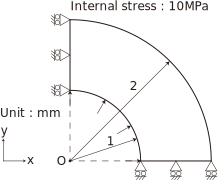
\includegraphics[keepaspectratio, scale = 0.85]
  {fig/内圧を受ける厚肉円筒モデル.ai}
  \caption{Analytical model of thick cylinder subjected to internal pressure}
  \label{fig:internal pressure}
\end{figure}

図~\ref{fig:internal pressure}に示すようにパラメータ空間を設定した.
2次の基底関数を用いた場合と3次の基底関数を用いた場合で,
パラメータ空間の各方向に対してコントロールポイント数が等しく,
一様オープンノットベクトルのIGA解析モデルをそれぞれ作成し,
各方向のコントロールポイントの分割数を変更したIGA解析モデルを作成した.
各方向のコントロールポイント数,自由度数,総要素数を表~\ref{table:ip}に示す.

\begin{table}[hbtp]
  \caption{Details of IGA analytical model}
  \label{table:ip}
  \centering
  \scalebox{0.95}{
    \begin{tabular}{|c|c|c|c|c|c|c|c|c|}
      \hline
      Order of basis function & \multicolumn{4}{c|}{2} & \multicolumn{4}{c|}{3} \\
      \hline
      Control points ($\xi \times \eta$) & $5\times 5$ & $10\times 10$ & $20\times 20$ & $40\times 40$ & $5\times 5$ & $10\times 10$ & $20\times 20$ & $40\times 40$ \\
      \hline
      Degrees of freedom & 40 & 180 & 760 & 3120 & 40 & 180 & 760 & 3120 \\
      \hline
      Total elements & 9 & 64 & 324 & 1444 & 4 & 49 & 289 & 1369 \\
      \hline
    \end{tabular}
  }
\end{table}

\newpage

例として,2次の基底関数と3次の基底関数で,各方向のコントロールポイント数が$5\times 5$のIGA解析モデルを
図~\ref{fig:iga order 2}及び図~\ref{fig:iga order 3}に示す.
点がコントロールポイント,実線が要素境界を表しており,
一様オープンノットベクトルを用いているため,各方向に等間隔の要素分割となっている.

\begin{figure}[htbp]
  \begin{tabular}{cc}
    \begin{minipage}[t]{0.45\hsize}
      \centering
      \includegraphics[keepaspectratio, scale=0.3]
      {fig/result_data_etc/iga/order2/model.png}
      \caption{An example of second-order analytical model (Control points $5\times 5$)}
      \label{fig:iga order 2}
    \end{minipage} &
    \begin{minipage}[t]{0.45\hsize}
      \centering
      \includegraphics[keepaspectratio, scale=0.3]
      {fig/result_data_etc/iga/order3/model.png}
      \caption{An example of third-order analytical model (Control points $5\times 5$)}
      \label{fig:iga order 3}
    \end{minipage}
  \end{tabular}
\end{figure}

\noindent
以上の解析モデルについて解析を行い,精度検証を行った.

内圧$P\ $MPaを受ける内径$2r_1\ $mm,外径$2r_2\ $mmの厚肉円筒の
応力の理論解は,円筒の中心を原点とした極座標表記で以下のように表される.

\begin{align}
  \sigma_{rr} &= -\frac{{r_1}^2{r_2}^2P}{{r_2}^2-{r_1}^2}\frac{1}{r^2}
              +\frac{{r_1}^2P}{{r_2}^2-{r_1}^2}\\
  \sigma_{\theta\theta} &= \frac{{r_1}^2{r_2}^2P}{{r_2}^2-{r_1}^2}\frac{1}{r^2}
                   +\frac{{r_1}^2P}{{r_2}^2-{r_1}^2}
\end{align}

\noindent
この理論解を用いて解析結果の誤差ノルムを算出し,
誤差精度の比較を行った.
誤差ノルムは以下のように定義した.

\begin{equation}
  {\rm{Error\ norm}} = \frac{\sqrt{\int_{\Omega}(\alpha_{\rm{analysis}}-\alpha_{\rm{theory}})^2 d\Omega}}{\sqrt{\int_{\Omega}{\alpha_{\rm{theory}}}^2 d\Omega}}
\end{equation}

\noindent
ここで,$\Omega$はIGA解析モデル全体の領域,
$\alpha$は比較パラメータである半径方向応力$\sigma_{rr}$,周方向応力$\sigma_{\theta\theta}$であり,
$\alpha_{\rm{theory}}$は比較パラメータの理論解,$\alpha_{\rm{analysis}}$は比較パラメータの解析結果の数値を表している.

\newpage

IGA解析結果の変位分布図を示す.
図~\ref{fig:iga 01}~図~\ref{fig:iga 04}は2次の基底関数と3次の基底関数の半径方向変位$u_{r}$である.

\begin{figure}[htbp]
  \begin{tabular}{cc}
    \begin{minipage}[t]{0.45\hsize}
      \centering
      \includegraphics[keepaspectratio, scale=0.3]
      {fig/result_data_etc/iga/order2/2_5x5.png}
      \caption{Displacement in r direction of second-order analytical model (Control points $5\times 5$)}
      \label{fig:iga 01}
    \end{minipage} &
    \begin{minipage}[t]{0.45\hsize}
      \centering
      \includegraphics[keepaspectratio, scale=0.3]
      {fig/result_data_etc/iga/order3/3_5x5.png}
      \caption{Displacement in r direction of third-order analytical model (Control points $5\times 5$)}
      \label{fig:iga 02}
    \end{minipage}
  \end{tabular}
\end{figure}

\begin{figure}[htbp]
  \begin{tabular}{cc}
    \begin{minipage}[t]{0.45\hsize}
      \centering
      \includegraphics[keepaspectratio, scale=0.3]
      {fig/result_data_etc/iga/order2/2_40x40.png}
      \caption{Displacement in r direction of second-order analytical model (Control points $40\times 40$)}
      \label{fig:iga 03}
    \end{minipage} &
    \begin{minipage}[t]{0.45\hsize}
      \centering
      \includegraphics[keepaspectratio, scale=0.3]
      {fig/result_data_etc/iga/order3/3_40x40.png}
      \caption{Displacement in r direction of third-order analytical model (Control points $40\times 40$)}
      \label{fig:iga 04}
    \end{minipage}
  \end{tabular}
\end{figure}

半径方向応力$\sigma_{rr}$と周方向応力$\sigma_{\theta\theta}$の誤差ノルムを算出し,
2次の基底関数を用いた場合と3次の基底関数を用いた場合の
自由度数と誤差ノルムの関係を両対数グラフで図~\ref{fig:iga ER 01},図~\ref{fig:iga ER 02}に示す.

\begin{figure}[htbp]
  \centering
  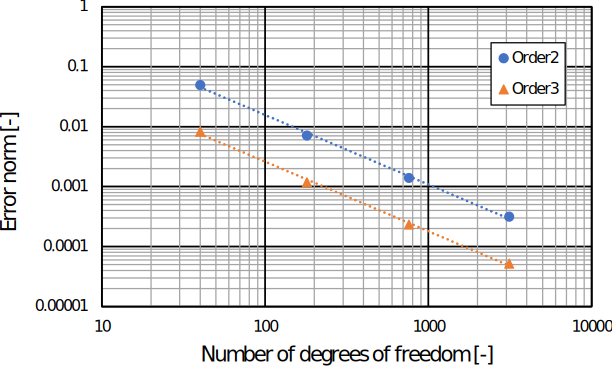
\includegraphics[keepaspectratio, scale = 0.8]
  {fig/result_data_etc/iga/ER01-crop.pdf}
  \caption{Error norm of $\sigma_{rr}$}
  \label{fig:iga ER 01}
\end{figure}

\begin{figure}[htbp]
  \centering
  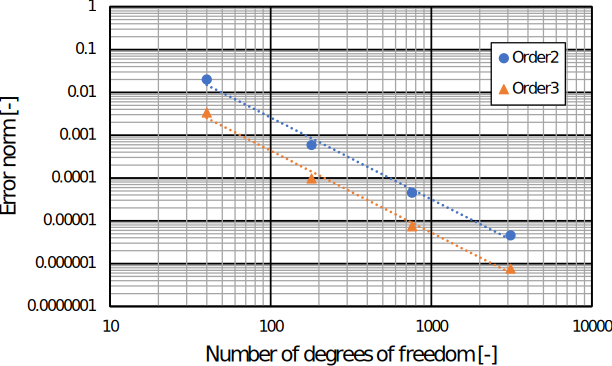
\includegraphics[keepaspectratio, scale = 0.8]
  {fig/result_data_etc/iga/ER02-crop.pdf}
  \caption{Error norm of $\sigma_{\theta\theta}$}
  \label{fig:iga ER 02}
\end{figure}

\newpage

\section{3次の基底関数を用いた重合パッチ法解析}
重合パッチ法解析を行い,2次と
3次の基底関数を用いた解析の誤差精度の検証を行った.

\subsection{遠方で一様引張を受ける円孔を有する平板の解析}

解析対象は,中央に半径$1\ $mmの円孔を有する遠方で一様引張を受ける平板であり,解析には二次元の$1/4$モデルを使用した.
解析問題を図~\ref{fig:GL}に示す.
平面ひずみ状態を仮定し,ヤング率は$206\ $GPa,ポアソン比は$0.3$とした.

\begin{figure}[htbp]
  \centering
  \includegraphics[keepaspectratio, scale = 0.85]
  {fig/GL.ai}
  \caption{Analytical model of plate with a circular hole}
  \label{fig:GL}
\end{figure}

\noindent
図~\ref{fig:GL}の問題は重合パッチ法では図~\ref{fig:G_and_L}に示す解析モデルと等価である.

\begin{figure}[htbp]
  \centering
  \includegraphics[keepaspectratio, scale = 0.85]
  {fig/G_and_L.ai}
  \caption{Analytical model of Global patch and Local patch}
  \label{fig:G_and_L}
\end{figure}

\newpage

\noindent
グローバルパッチはシンプルな形状を作成し,一様引張と対称性を表すための変位固定の境界条件を設定した.
ローカルパッチは円孔を表現する詳細形状を作成し,グローバルパッチ上のローカルパッチの境界$\Gamma^{GL}$で変位固定を行った.

数値積分には各方向の積分点数が$4\times 4$のガウス・ルジャンドル積分法を用いた.
ただし,ローカルパッチの1要素がグローバルパッチの2要素以上を跨ぐ場合では
被積分関数がグローバルパッチの要素境界で連続性が低下し,
結合剛性マトリクスの積分精度が低下することが確認されており,
該当するローカルパッチについては積分点数を$10\times 10$として積分を行った.

図~\ref{fig:G_and_L}に示すようにパラメータ空間を設定した.
ノットベクトルは一様オープンノットベクトルを用いた.

無限遠にて一様引張応力$\sigma_0$を受ける場合の理論解は円孔の中心を原点とする極座標表記を用いて以下のように表される.

\begin{align}
  \sigma_{rr} &= \frac{\sigma_0}{2}\left(1 - \frac{\rho^2}{r^2}\right) - \frac{\sigma_0}{2}\left(1 - \frac{4\rho^2}{r^2} + \frac{3\rho^4}{r^4}\right)\cos{2\theta}\\
  \sigma_{\theta\theta} &= \frac{\sigma_0}{2}\left(1 + \frac{\rho^2}{r^2}\right) + \frac{\sigma_0}{2} \left( 1 + \frac{3\rho^4}{r^4} \right) \cos{2\theta}\\
  \tau_{r\theta} &= \frac{\sigma_0}{2} \left( 1 + \frac{2\rho^2}{r^2} - \frac{3\rho^4}{r^4} \right)
\end{align}

\noindent
また,直交座標系から極座標系への座標変換は以下のように表される.

\begin{align}
  \sigma_{rr} &= \sigma_{xx} \cos^2\theta + \sigma_{yy} \sin^2\theta + 2\tau_{xy} \sin\theta \cos\theta \\
  \sigma_{\theta\theta} &= \sigma_{xx} \sin^2\theta + \sigma_{yy} \cos^2\theta - 2\tau_{xy} \cos\theta \sin\theta \\
  \tau_{r\theta} &= (\sigma_{yy} - \sigma_{xx}) \sin\theta \cos\theta + \tau_{xy}(\cos^2\theta - \sin^2\theta)
\end{align}

\noindent
この理論解を用いて解析結果の誤差ノルムを以下のように定義する.

\begin{equation}
  {\rm{Error\ norm}} = \frac{\sqrt{\int_{\Omega^L}(\alpha_{\rm{analysis}}-\alpha_{\rm{theory}})^2 d\Omega}}{\sqrt{\int_{\Omega^L}{\alpha_{\rm{theory}}}^2 d\Omega}}
\end{equation}

\noindent
ここで,$\Omega^L$は重合パッチ法解析モデルにおけるローカルパッチの領域,
$\alpha$は比較パラメータである半径方向応力$\sigma_{rr}$,周方向応力$\sigma_{\theta\theta}$であり,
$\alpha_{\rm{theory}}$は比較パラメータの理論解,$\alpha_{\rm{analysis}}$は比較パラメータの解析結果の数値を表している.

\subsubsection{各パッチでの基底関数の次数の組み合わせによる解析精度検証}
表~\ref{table:combination}に示すようにグローバルパッチとローカルパッチをそれぞれ2次の基底関数,3次の基底関数で作成し,
その組み合わせの違いによる誤差精度を検証した.
さらに表~\ref{table:GL_division}に示すように各組み合わせでグローバルパッチの分割数を固定して,ローカルパッチの分割数を変更した.

\begin{table}[hbtp]
  \caption{Combination of order of basis function}
  \label{table:combination}
  \centering
  \scalebox{1.0}{
    \begin{tabular}{|c|c|c|}
      \hline
       &
      \begin{tabular}{c}
        Order of basis function \\
        on Global patch
      \end{tabular} &
      \begin{tabular}{c}
        Order of basis function \\
        on Local patch
      \end{tabular} \\
      \hline
      (a) Order(2, 2) & 2 & 2 \\
      \hline
      (b) Order(2, 3) & 2 & 3 \\
      \hline
      (c) Order(3, 2) & 3 & 2 \\
      \hline
      (d) Order(3, 3) & 3 & 3 \\
      \hline
    \end{tabular}
  }
\end{table}

\begin{table}[hbtp]
  \caption{Control points on Global patch and Local patch}
  \label{table:GL_division}
  \centering
  \scalebox{1.0}{
    \begin{tabular}{|c|c|c|c|c|}
      \hline
      \begin{tabular}{c}
        Control points\\
        on Global patch ($\xi \times \eta$)
      \end{tabular} & \multicolumn{4}{c|}{$30\times 30$} \\
      \hline
      \begin{tabular}{c}
        Control points\\
        on Local patch ($\xi \times \eta$)
      \end{tabular} & $5\times 5$ & $10\times 10$ & $20\times 20$ & $30\times 30$ \\
      \hline
    \end{tabular}
  }
\end{table}

例として,各組み合わせでローカルパッチの各方向のコントロールポイント数が$5\times 5$の重合パッチ法解析モデルを
図~\ref{fig:22}及び図~\ref{fig:33}に示す.

\begin{figure}[htbp]
  \begin{tabular}{cc}
    \begin{minipage}[t]{0.45\hsize}
      \centering
      \includegraphics[keepaspectratio, scale=0.3]
      {fig/result_data_etc/s-iga01/model/22.png}
      \caption{An example of (a) analytical model (Order(2, 2), Control points on Local patch $5\times 5$)}
      \label{fig:22}
    \end{minipage} &
    \begin{minipage}[t]{0.45\hsize}
      \centering
      \includegraphics[keepaspectratio, scale=0.3]
      {fig/result_data_etc/s-iga01/model/23.png}
      \caption{An example of (b) analytical model (Order(2, 3), Control points on Local patch $5\times 5$)}
      \label{fig:23}
    \end{minipage}
  \end{tabular}
\end{figure}

\newpage

\begin{figure}[htbp]
  \begin{tabular}{cc}
    \begin{minipage}[t]{0.45\hsize}
      \centering
      \includegraphics[keepaspectratio, scale=0.3]
      {fig/result_data_etc/s-iga01/model/32.png}
      \caption{An example of (c) analytical model (Order(3, 2), Control points on Local patch $5\times 5$)}
      \label{fig:32}
    \end{minipage} &
    \begin{minipage}[t]{0.45\hsize}
      \centering
      \includegraphics[keepaspectratio, scale=0.3]
      {fig/result_data_etc/s-iga01/model/33.png}
      \caption{An example of (d) analytical model (Order(3, 3), Control points on Local patch $5\times 5$)}
      \label{fig:33}
    \end{minipage}
  \end{tabular}
\end{figure}

\noindent
以上の解析モデルについて解析を行い,精度検証を行った.
半径方向応力$\sigma_{rr}$と周方向応力$\sigma_{\theta\theta}$の自由度と誤差ノルムの関係を
図~\ref{fig:ERNr},図~\ref{fig:ERNt}に示す.

\begin{figure}[htbp]
  \centering
  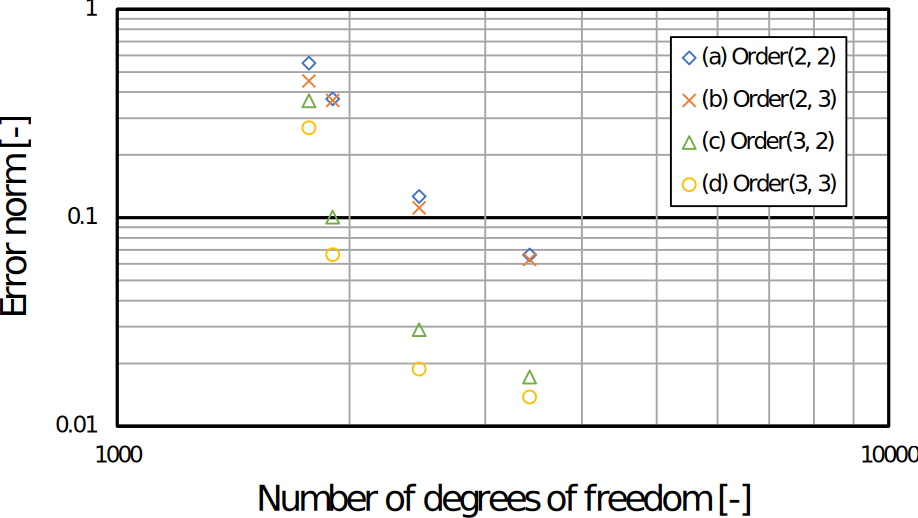
\includegraphics[keepaspectratio, scale=0.5]
  {fig/result_data_etc/s-iga01/r-crop.pdf}
  \caption{Error norm of $\sigma_{rr}$ in each case}
  \label{fig:ERNr}
\end{figure}

\newpage

\begin{figure}[htbp]
  \centering
  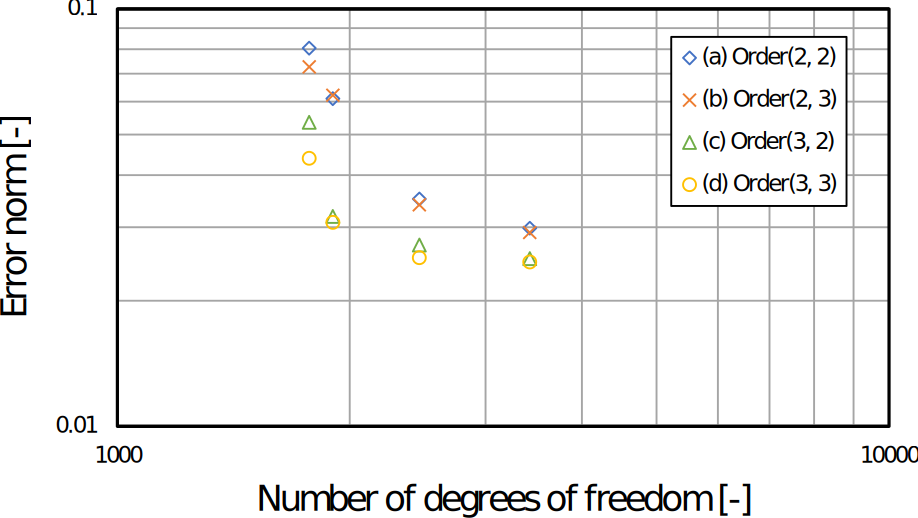
\includegraphics[keepaspectratio, scale=0.5]
  {fig/result_data_etc/s-iga01/theta-crop.pdf}
  \caption{Error norm of $\sigma_{\theta\theta}$ in each case}
  \label{fig:ERNt}
\end{figure}

$y$方向応力$\sigma_{yy}$の応力分布図を図~\ref{fig:contour22}~図~\ref{fig:contour33}に示す.

\begin{figure}[htbp]
  \begin{tabular}{cc}
    \begin{minipage}[t]{0.45\hsize}
      \centering
      \includegraphics[keepaspectratio, scale=0.3]
      {fig/result_data_etc/s-iga01/contour/2_2.png}
      \caption{Stress in $y$ direction on Local patch ((a) Order(2, 2), Control points on Local patch $30\times 30$)}
      \label{fig:contour22}
    \end{minipage} &
    \begin{minipage}[t]{0.45\hsize}
      \centering
      \includegraphics[keepaspectratio, scale=0.3]
      {fig/result_data_etc/s-iga01/contour/2_3.png}
      \caption{Stress in $y$ direction on Local patch ((b) Order(2, 3), Control points on Local patch $30\times 30$)}
      \label{fig:contour23}
    \end{minipage}
  \end{tabular}
\end{figure}

\newpage

\begin{figure}[htbp]
  \begin{tabular}{cc}
    \begin{minipage}[t]{0.45\hsize}
      \centering
      \includegraphics[keepaspectratio, scale=0.3]
      {fig/result_data_etc/s-iga01/contour/3_2.png}
      \caption{Stress in $y$ direction on Local patch ((c) Order(3, 2), Control points on Local patch $30\times 30$)}
      \label{fig:contour32}
    \end{minipage} &
    \begin{minipage}[t]{0.45\hsize}
      \centering
      \includegraphics[keepaspectratio, scale=0.3]
      {fig/result_data_etc/s-iga01/contour/3_3.png}
      \caption{Stress in $y$ direction on Local patch ((d) Order(3, 3), Control points on Local patch $30\times 30$)}
      \label{fig:contour33}
    \end{minipage}
  \end{tabular}
\end{figure}

\newpage

\subsubsection{グローバルパッチの分割数を固定してローカルパッチの分割数を変更した解析}
グローバルパッチのコントロールポイントの分割数を固定してローカルパッチのコントロールポイントの分割数を
変更した重合パッチ法解析を行った.
グローバルパッチとローカルパッチの基底関数が共に2次の場合と共に3次の場合で解析を行い比較した.
グローバルパッチとローカルパッチは
2次の基底関数を用いた場合と3次の基底関数を用いた場合で,
パラメータ空間の各方向に対してコントロールポイント数が等しく,
各方向のコントロールポイントの分割数を変更した重合パッチ法解析モデルを作成した.
グローバルパッチとローカルパッチの各方向のコントロールポイント数,自由度数,総要素数を表~\ref{table:G fixed}に示す.

\begin{table}[hbtp]
  \caption{Details of S-IGA analytical model (Global patch division is fixed)}
  \label{table:G fixed}
  \centering
  \scalebox{0.8}{
    \begin{tabular}{|c|c|c|c|c|c|c|c|c|}
      \hline
      \begin{tabular}{c}
        Order of basis function \\
        (Global patch and Local patch)
      \end{tabular} & \multicolumn{4}{c|}{2} & \multicolumn{4}{c|}{3} \\
      \hline
      \begin{tabular}{c}
        Control points\\
        on Global patch ($\xi \times \eta$)
      \end{tabular} & \multicolumn{4}{c|}{$30\times 30$} & \multicolumn{4}{c|}{$30\times 30$} \\
      \hline
      \begin{tabular}{c}
        Control points\\
        on Local patch ($\xi \times \eta$)
      \end{tabular} & $5\times 5$ & $10\times 10$ & $20\times 20$ & $30\times 30$ & $5\times 5$ & $10\times 10$ & $20\times 20$ & $30\times 30$ \\
      \hline
      Degrees of freedom & 1772 & 1902 & 2462 & 3422 & 1772 & 1902 & 2462 & 3422 \\
      \hline
      Total elements & 793 & 848 & 1108 & 1568 & 733 & 778 & 1018 & 1458 \\
      \hline
    \end{tabular}
  }
\end{table}

例として,2次の基底関数で,ローカルパッチの分割数を変更した重合パッチ法解析モデルを図~\ref{fig:s-iga02 model01}~
図~\ref{fig:s-iga02 model04}に示す.

\begin{figure}[htbp]
  \begin{tabular}{cc}
    \begin{minipage}[t]{0.45\hsize}
      \centering
      \includegraphics[keepaspectratio, scale=0.3]
      {fig/result_data_etc/s-iga02/model/5x5.png}
      \caption{An example of second-order S-IGA analytical model (Global patch $30\times 30$, Local patch $5\times 5$)}
      \label{fig:s-iga02 model01}
    \end{minipage} &
    \begin{minipage}[t]{0.45\hsize}
      \centering
      \includegraphics[keepaspectratio, scale=0.3]
      {fig/result_data_etc/s-iga02/model/10x10.png}
      \caption{An example of second-order S-IGA analytical model (Global patch $30\times 30$, Local patch $10\times 10$)}
      \label{fig:s-iga02 model02}
    \end{minipage}
  \end{tabular}
\end{figure}

\newpage

\begin{figure}[hbtp]
  \begin{tabular}{cc}
    \begin{minipage}[t]{0.45\hsize}
      \centering
      \includegraphics[keepaspectratio, scale=0.3]
      {fig/result_data_etc/s-iga02/model/20x20.png}
      \caption{An example of second-order S-IGA analytical model (Global patch $30\times 30$, Local patch $20\times 20$)}
      \label{fig:s-iga02 model03}
    \end{minipage} &
    \begin{minipage}[t]{0.45\hsize}
      \centering
      \includegraphics[keepaspectratio, scale=0.3]
      {fig/result_data_etc/s-iga02/model/30x30.png}
      \caption{An example of second-order S-IGA analytical model (Global patch $30\times 30$, Local patch $30\times 30$)}
      \label{fig:s-iga02 model04}
    \end{minipage}
  \end{tabular}
\end{figure}

\noindent
以上の解析モデルについて解析を行い,精度検証を行った.
円孔縁の主応力$\sigma_1, \sigma_2$の分布,$x$軸上の$y$方向応力$\sigma_{yy}$,応力分布図を比較し,
ローカルパッチの分割数による影響を比較した.

円孔縁の主応力$\sigma_1, \sigma_2$の分布を
図~\ref{fig:s-iga02 s 2 5x5}~図~\ref{fig:s-iga02 s 3 30x30}に示す.

\begin{figure}[hbtp]
  \begin{tabular}{cc}
    \begin{minipage}[t]{0.45\hsize}
      \centering
      \includegraphics[keepaspectratio, scale=0.4]
      {fig/result_data_etc/s-iga02/order2/s_5x5-crop.pdf}
      \caption{Principal stress along the periphery of the circular hole (second-order, Global patch $30\times 30$, Local patch $5\times 5$)}
      \label{fig:s-iga02 s 2 5x5}
    \end{minipage} &
    \begin{minipage}[t]{0.45\hsize}
      \centering
      \includegraphics[keepaspectratio, scale=0.4]
      {fig/result_data_etc/s-iga02/order3/s_5x5-crop.pdf}
      \caption{Principal stress along the periphery of the circular hole (third-order, Global patch $30\times 30$, Local patch $5\times 5$)}
      \label{fig:s-iga02 s 3 5x5}
    \end{minipage}
  \end{tabular}
\end{figure}

\newpage

\begin{figure}[hbtp]
  \begin{tabular}{cc}
    \begin{minipage}[t]{0.45\hsize}
      \centering
      \includegraphics[keepaspectratio, scale=0.4]
      {fig/result_data_etc/s-iga02/order2/s_10x10-crop.pdf}
      \caption{Principal stress along the periphery of the circular hole (second-order, Global patch $30\times 30$, Local patch $10\times 10$)}
      \label{fig:s-iga02 s 2 10x10}
    \end{minipage} &
    \begin{minipage}[t]{0.45\hsize}
      \centering
      \includegraphics[keepaspectratio, scale=0.4]
      {fig/result_data_etc/s-iga02/order3/s_10x10-crop.pdf}
      \caption{Principal stress along the periphery of the circular hole (third-order, Global patch $30\times 30$, Local patch $10\times 10$)}
      \label{fig:s-iga02 s 3 10x10}
    \end{minipage}
  \end{tabular}
\end{figure}

\begin{figure}[hbtp]
  \begin{tabular}{cc}
    \begin{minipage}[t]{0.45\hsize}
      \centering
      \includegraphics[keepaspectratio, scale=0.4]
      {fig/result_data_etc/s-iga02/order2/s_20x20-crop.pdf}
      \caption{Principal stress along the periphery of the circular hole (second-order, Global patch $30\times 30$, Local patch $20\times 20$)}
      \label{fig:s-iga02 s 2 20x20}
    \end{minipage} &
    \begin{minipage}[t]{0.45\hsize}
      \centering
      \includegraphics[keepaspectratio, scale=0.4]
      {fig/result_data_etc/s-iga02/order3/s_20x20-crop.pdf}
      \caption{Principal stress along the periphery of the circular hole (third-order, Global patch $30\times 30$, Local patch $20\times 20$)}
      \label{fig:s-iga02 s 3 20x20}
    \end{minipage}
  \end{tabular}
\end{figure}

\begin{figure}[hbtp]
  \begin{tabular}{cc}
    \begin{minipage}[t]{0.45\hsize}
      \centering
      \includegraphics[keepaspectratio, scale=0.4]
      {fig/result_data_etc/s-iga02/order2/s_30x30-crop.pdf}
      \caption{Principal stress along the periphery of the circular hole (second-order, Global patch $30\times 30$, Local patch $30\times 30$)}
      \label{fig:s-iga02 s 2 30x30}
    \end{minipage} &
    \begin{minipage}[t]{0.45\hsize}
      \centering
      \includegraphics[keepaspectratio, scale=0.4]
      {fig/result_data_etc/s-iga02/order3/s_30x30-crop.pdf}
      \caption{Principal stress along the periphery of the circular hole (third-order, Global patch $30\times 30$, Local patch $30\times 30$)}
      \label{fig:s-iga02 s 3 30x30}
    \end{minipage}
  \end{tabular}
\end{figure}

\newpage

$x$軸上の$y$方向応力$\sigma_{yy}$を
図~\ref{fig:s-iga02 y 2 5x5}~図~\ref{fig:s-iga02 y 3 30x30}に示す.

\begin{figure}[hbtp]
  \begin{tabular}{cc}
    \begin{minipage}[t]{0.45\hsize}
      \centering
      \includegraphics[keepaspectratio, scale=0.4]
      {fig/result_data_etc/s-iga02/order2/y_5x5-crop.pdf}
      \caption{Stress in $y$ direction along the line $y = 0$ (second-order, Global patch $30\times 30$, Local patch $5\times 5$)}
      \label{fig:s-iga02 y 2 5x5}
    \end{minipage} &
    \begin{minipage}[t]{0.45\hsize}
      \centering
      \includegraphics[keepaspectratio, scale=0.4]
      {fig/result_data_etc/s-iga02/order3/y_5x5-crop.pdf}
      \caption{Stress in $y$ direction along the line $y = 0$ (third-order, Global patch $30\times 30$, Local patch $5\times 5$)}
      \label{fig:s-iga02 y 3 5x5}
    \end{minipage}
  \end{tabular}
\end{figure}

\begin{figure}[hbtp]
  \begin{tabular}{cc}
    \begin{minipage}[t]{0.45\hsize}
      \centering
      \includegraphics[keepaspectratio, scale=0.4]
      {fig/result_data_etc/s-iga02/order2/y_10x10-crop.pdf}
      \caption{Stress in $y$ direction along the line $y = 0$ (second-order, Global patch $30\times 30$, Local patch $10\times 10$)}
      \label{fig:s-iga02 y 2 10x10}
    \end{minipage} &
    \begin{minipage}[t]{0.45\hsize}
      \centering
      \includegraphics[keepaspectratio, scale=0.4]
      {fig/result_data_etc/s-iga02/order3/y_10x10-crop.pdf}
      \caption{Stress in $y$ direction along the line $y = 0$ (third-order, Global patch $30\times 30$, Local patch $10\times 10$)}
      \label{fig:s-iga02 y 3 10x10}
    \end{minipage}
  \end{tabular}
\end{figure}

\begin{figure}[hbtp]
  \begin{tabular}{cc}
    \begin{minipage}[t]{0.45\hsize}
      \centering
      \includegraphics[keepaspectratio, scale=0.4]
      {fig/result_data_etc/s-iga02/order2/y_20x20-crop.pdf}
      \caption{Stress in $y$ direction along the line $y = 0$ (second-order, Global patch $30\times 30$, Local patch $20\times 20$)}
      \label{fig:s-iga02 y 2 20x20}
    \end{minipage} &
    \begin{minipage}[t]{0.45\hsize}
      \centering
      \includegraphics[keepaspectratio, scale=0.4]
      {fig/result_data_etc/s-iga02/order3/y_20x20-crop.pdf}
      \caption{Stress in $y$ direction along the line $y = 0$ (third-order, Global patch $30\times 30$, Local patch $20\times 20$)}
      \label{fig:s-iga02 y 3 20x20}
    \end{minipage}
  \end{tabular}
\end{figure}

\newpage

\begin{figure}[hbtp]
  \begin{tabular}{cc}
    \begin{minipage}[t]{0.45\hsize}
      \centering
      \includegraphics[keepaspectratio, scale=0.4]
      {fig/result_data_etc/s-iga02/order2/y_30x30-crop.pdf}
      \caption{Stress in $y$ direction along the line $y = 0$ (second-order, Global patch $30\times 30$, Local patch $30\times 30$)}
      \label{fig:s-iga02 y 2 30x30}
    \end{minipage} &
    \begin{minipage}[t]{0.45\hsize}
      \centering
      \includegraphics[keepaspectratio, scale=0.4]
      {fig/result_data_etc/s-iga02/order3/y_30x30-crop.pdf}
      \caption{Stress in $y$ direction along the line $y = 0$ (third-order, Global patch $30\times 30$, Local patch $30\times 30$)}
      \label{fig:s-iga02 y 3 30x30}
    \end{minipage}
  \end{tabular}
\end{figure}

$y$方向応力$\sigma_{yy}$の分布図を図~\ref{fig:s-iga02 y 2},図~\ref{fig:s-iga02 y 3}に示す.

\begin{figure}[hbtp]
  \begin{tabular}{cc}
    \begin{minipage}[t]{0.45\hsize}
      \centering
      \includegraphics[keepaspectratio, scale=0.3]
      {fig/result_data_etc/s-iga02/contour/2.png}
      \caption{Stress in $y$ direction on Local patch (second-order, Global patch $30\times 30$, Local patch $20\times 20$)}
      \label{fig:s-iga02 y 2}
    \end{minipage} &
    \begin{minipage}[t]{0.45\hsize}
      \centering
      \includegraphics[keepaspectratio, scale=0.3]
      {fig/result_data_etc/s-iga02/contour/3.png}
      \caption{Stress in $y$ direction on Local patch (third-order, Global patch $30\times 30$, Local patch $20\times 20$)}
      \label{fig:s-iga02 y 3}
    \end{minipage}
  \end{tabular}
\end{figure}

\newpage

\subsubsection{ローカルパッチの分割数を固定してグローバルパッチの分割数を変更した解析}
ローカルパッチのコントロールポイントの分割数を固定してグローバルパッチのコントロールポイントの分割数を
変更した重合パッチ法解析を行った.
グローバルパッチとローカルパッチの基底関数が共に2次の場合と共に3次の場合で解析を行い比較した.
グローバルパッチとローカルパッチは
2次の基底関数を用いた場合と3次の基底関数を用いた場合で,
パラメータ空間の各方向に対してコントロールポイント数が等しく,
各方向のコントロールポイントの分割数を変更した重合パッチ法解析モデルを作成した.
グローバルパッチとローカルパッチの各方向のコントロールポイント数,自由度数,総要素数を表~\ref{table:L fixed}に示す.

\begin{table}[hbtp]
  \caption{Details of S-IGA analytical model (Local patch division is fixed)}
  \label{table:L fixed}
  \centering
  \scalebox{0.8}{
    \begin{tabular}{|c|c|c|c|c|c|c|c|c|}
      \hline
      \begin{tabular}{c}
        Order of basis function \\
        (Global patch and Local patch)
      \end{tabular} & \multicolumn{4}{c|}{2} & \multicolumn{4}{c|}{3} \\
      \hline
      \begin{tabular}{c}
        Control points\\
        on Local patch ($\xi \times \eta$)
      \end{tabular} & \multicolumn{4}{c|}{$30\times 30$} & \multicolumn{4}{c|}{$30\times 30$} \\
      \hline
      \begin{tabular}{c}
        Control points\\
        on Global patch ($\xi \times \eta$)
      \end{tabular} & $5\times 5$ & $10\times 10$ & $20\times 20$ & $30\times 30$ & $5\times 5$ & $10\times 10$ & $20\times 20$ & $30\times 30$ \\
      \hline
      Degrees of freedom & 1722 & 1862 & 2442 & 3422 & 1722 & 1862 & 2442 & 3422 \\
      \hline
      Total elements & 793 & 848 & 1108 & 1568 & 733 & 778 & 1018 & 1458 \\
      \hline
    \end{tabular}
  }
\end{table}

例として,2次の基底関数で,グローバルパッチの分割数を変更した重合パッチ法解析モデルを図~\ref{fig:s-iga03 model01}~
図~\ref{fig:s-iga03 model04}に示す.

\begin{figure}[htbp]
  \begin{tabular}{cc}
    \begin{minipage}[t]{0.45\hsize}
      \centering
      \includegraphics[keepaspectratio, scale=0.3]
      {fig/result_data_etc/s-iga03/model/5x5.png}
      \caption{An example of second-order S-IGA analytical model (Global patch $5\times 5$, Local patch $30\times 30$)}
      \label{fig:s-iga03 model01}
    \end{minipage} &
    \begin{minipage}[t]{0.45\hsize}
      \centering
      \includegraphics[keepaspectratio, scale=0.3]
      {fig/result_data_etc/s-iga03/model/10x10.png}
      \caption{An example of second-order S-IGA analytical model (Global patch $10\times 10$, Local patch $30\times 30$)}
      \label{fig:s-iga03 model02}
    \end{minipage}
  \end{tabular}
\end{figure}

\newpage

\begin{figure}[htbp]
  \begin{tabular}{cc}
    \begin{minipage}[t]{0.45\hsize}
      \centering
      \includegraphics[keepaspectratio, scale=0.3]
      {fig/result_data_etc/s-iga03/model/20x20.png}
      \caption{An example of second-order S-IGA analytical model (Global patch $20\times 20$, Local patch $30\times 30$)}
      \label{fig:s-iga03 model03}
    \end{minipage} &
    \begin{minipage}[t]{0.45\hsize}
      \centering
      \includegraphics[keepaspectratio, scale=0.3]
      {fig/result_data_etc/s-iga03/model/30x30.png}
      \caption{An example of second-order S-IGA analytical model (Global patch $30\times 30$, Local patch $30\times 30$)}
      \label{fig:s-iga03 model04}
    \end{minipage}
  \end{tabular}
\end{figure}

\noindent
以上の解析モデルについて解析を行い,精度検証を行った.
円孔縁の主応力$\sigma_1, \sigma_2$の分布,$x$軸上の$y$方向応力$\sigma_{yy}$,応力分布図を比較し,
グローバルパッチの分割数による影響を比較した.

円孔縁の主応力$\sigma_1, \sigma_2$の分布を
図~\ref{fig:s-iga03 s 2 5x5}~図~\ref{fig:s-iga03 s 3 30x30}に示す.

\begin{figure}[hbtp]
  \begin{tabular}{cc}
    \begin{minipage}[t]{0.45\hsize}
      \centering
      \includegraphics[keepaspectratio, scale=0.4]
      {fig/result_data_etc/s-iga03/order2/s_5x5-crop.pdf}
      \caption{Principal stress along the periphery of the circular hole (second-order, Global patch $5\times 5$, Local patch $30\times 30$)}
      \label{fig:s-iga03 s 2 5x5}
    \end{minipage} &
    \begin{minipage}[t]{0.45\hsize}
      \centering
      \includegraphics[keepaspectratio, scale=0.4]
      {fig/result_data_etc/s-iga03/order3/s_5x5-crop.pdf}
      \caption{Principal stress along the periphery of the circular hole (third-order, Global patch $5\times 5$, Local patch $30\times 30$)}
      \label{fig:s-iga03 s 3 5x5}
    \end{minipage}
  \end{tabular}
\end{figure}

\newpage

\begin{figure}[hbtp]
  \begin{tabular}{cc}
    \begin{minipage}[t]{0.45\hsize}
      \centering
      \includegraphics[keepaspectratio, scale=0.4]
      {fig/result_data_etc/s-iga03/order2/s_10x10-crop.pdf}
      \caption{Principal stress along the periphery of the circular hole (second-order, Global patch $10\times 10$, Local patch $30\times 30$)}
      \label{fig:s-iga03 s 2 10x10}
    \end{minipage} &
    \begin{minipage}[t]{0.45\hsize}
      \centering
      \includegraphics[keepaspectratio, scale=0.4]
      {fig/result_data_etc/s-iga03/order3/s_10x10-crop.pdf}
      \caption{Principal stress along the periphery of the circular hole (third-order, Global patch $10\times 10$, Local patch $30\times 30$)}
      \label{fig:s-iga03 s 3 10x10}
    \end{minipage}
  \end{tabular}
\end{figure}

\begin{figure}[hbtp]
  \begin{tabular}{cc}
    \begin{minipage}[t]{0.45\hsize}
      \centering
      \includegraphics[keepaspectratio, scale=0.4]
      {fig/result_data_etc/s-iga03/order2/s_20x20-crop.pdf}
      \caption{Principal stress along the periphery of the circular hole (second-order, Global patch $20\times 20$, Local patch $30\times 30$)}
      \label{fig:s-iga03 s 2 20x20}
    \end{minipage} &
    \begin{minipage}[t]{0.45\hsize}
      \centering
      \includegraphics[keepaspectratio, scale=0.4]
      {fig/result_data_etc/s-iga03/order3/s_20x20-crop.pdf}
      \caption{Principal stress along the periphery of the circular hole (third-order, Global patch $20\times 20$, Local patch $30\times 30$)}
      \label{fig:s-iga03 s 3 20x20}
    \end{minipage}
  \end{tabular}
\end{figure}

\begin{figure}[hbtp]
  \begin{tabular}{cc}
    \begin{minipage}[t]{0.45\hsize}
      \centering
      \includegraphics[keepaspectratio, scale=0.4]
      {fig/result_data_etc/s-iga03/order2/s_30x30-crop.pdf}
      \caption{Principal stress along the periphery of the circular hole (second-order, Global patch $30\times 30$, Local patch $30\times 30$)}
      \label{fig:s-iga03 s 2 30x30}
    \end{minipage} &
    \begin{minipage}[t]{0.45\hsize}
      \centering
      \includegraphics[keepaspectratio, scale=0.4]
      {fig/result_data_etc/s-iga03/order3/s_30x30-crop.pdf}
      \caption{Principal stress along the periphery of the circular hole (third-order, Global patch $30\times 30$, Local patch $30\times 30$)}
      \label{fig:s-iga03 s 3 30x30}
    \end{minipage}
  \end{tabular}
\end{figure}

\newpage

$x$軸上の$y$方向応力$\sigma_{yy}$を
図~\ref{fig:s-iga03 y 2 5x5}~図~\ref{fig:s-iga03 y 3 30x30}に示す.

\begin{figure}[hbtp]
  \begin{tabular}{cc}
    \begin{minipage}[t]{0.45\hsize}
      \centering
      \includegraphics[keepaspectratio, scale=0.4]
      {fig/result_data_etc/s-iga03/order2/y_5x5-crop.pdf}
      \caption{Stress in $y$ direction along the line $y = 0$ (second-order, Global patch $5\times 5$, Local patch $30\times 30$)}
      \label{fig:s-iga03 y 2 5x5}
    \end{minipage} &
    \begin{minipage}[t]{0.45\hsize}
      \centering
      \includegraphics[keepaspectratio, scale=0.4]
      {fig/result_data_etc/s-iga03/order3/y_5x5-crop.pdf}
      \caption{Stress in $y$ direction along the line $y = 0$ (third-order, Global patch $5\times 5$, Local patch $30\times 30$)}
      \label{fig:s-iga03 y 3 5x5}
    \end{minipage}
  \end{tabular}
\end{figure}

\begin{figure}[hbtp]
  \begin{tabular}{cc}
    \begin{minipage}[t]{0.45\hsize}
      \centering
      \includegraphics[keepaspectratio, scale=0.4]
      {fig/result_data_etc/s-iga03/order2/y_10x10-crop.pdf}
      \caption{Stress in $y$ direction along the line $y = 0$ (second-order, Global patch $10\times 10$, Local patch $30\times 30$)}
      \label{fig:s-iga03 y 2 10x10}
    \end{minipage} &
    \begin{minipage}[t]{0.45\hsize}
      \centering
      \includegraphics[keepaspectratio, scale=0.4]
      {fig/result_data_etc/s-iga03/order3/y_10x10-crop.pdf}
      \caption{Stress in $y$ direction along the line $y = 0$ (third-order, Global patch $10\times 10$, Local patch $30\times 30$)}
      \label{fig:s-iga03 y 3 10x10}
    \end{minipage}
  \end{tabular}
\end{figure}

\begin{figure}[hbtp]
  \begin{tabular}{cc}
    \begin{minipage}[t]{0.45\hsize}
      \centering
      \includegraphics[keepaspectratio, scale=0.4]
      {fig/result_data_etc/s-iga03/order2/y_20x20-crop.pdf}
      \caption{Stress in $y$ direction along the line $y = 0$ (second-order, Global patch $20\times 20$, Local patch $30\times 30$)}
      \label{fig:s-iga03 y 2 20x20}
    \end{minipage} &
    \begin{minipage}[t]{0.45\hsize}
      \centering
      \includegraphics[keepaspectratio, scale=0.4]
      {fig/result_data_etc/s-iga03/order3/y_20x20-crop.pdf}
      \caption{Stress in $y$ direction along the line $y = 0$ (third-order, Global patch $20\times 20$, Local patch $30\times 30$)}
      \label{fig:s-iga03 y 3 20x20}
    \end{minipage}
  \end{tabular}
\end{figure}

\newpage

\begin{figure}[hbtp]
  \begin{tabular}{cc}
    \begin{minipage}[t]{0.45\hsize}
      \centering
      \includegraphics[keepaspectratio, scale=0.4]
      {fig/result_data_etc/s-iga03/order2/y_30x30-crop.pdf}
      \caption{Stress in $y$ direction along the line $y = 0$ (second-order, Global patch $30\times 30$, Local patch $30\times 30$)}
      \label{fig:s-iga03 y 2 30x30}
    \end{minipage} &
    \begin{minipage}[t]{0.45\hsize}
      \centering
      \includegraphics[keepaspectratio, scale=0.4]
      {fig/result_data_etc/s-iga03/order3/y_30x30-crop.pdf}
      \caption{Stress in $y$ direction along the line $y = 0$ (third-order, Global patch $30\times 30$, Local patch $30\times 30$)}
      \label{fig:s-iga03 y 3 30x30}
    \end{minipage}
  \end{tabular}
\end{figure}

$y$方向応力$\sigma_{yy}$の分布図を図~\ref{fig:s-iga03 y 2},図~\ref{fig:s-iga03 y 3}に示す.

\begin{figure}[hbtp]
  \begin{tabular}{cc}
    \begin{minipage}[t]{0.45\hsize}
      \centering
      \includegraphics[keepaspectratio, scale=0.3]
      {fig/result_data_etc/s-iga03/contour/2.png}
      \caption{Stress in $y$ direction on Local patch (second-order, Global patch $20\times 20$, Local patch $30\times 30$)}
      \label{fig:s-iga03 y 2}
    \end{minipage} &
    \begin{minipage}[t]{0.45\hsize}
      \centering
      \includegraphics[keepaspectratio, scale=0.3]
      {fig/result_data_etc/s-iga03/contour/3.png}
      \caption{Stress in $y$ direction on Local patch (third-order, Global patch $20\times 20$, Local patch $30\times 30$)}
      \label{fig:s-iga03 y 3}
    \end{minipage}
  \end{tabular}
\end{figure}

\newpage

\subsubsection{グローバルパッチの分割数を固定してローカルパッチのサイズと分割数を変更した解析}
グローバルパッチのコントロールポイントの分割数を固定してローカルパッチの全体のサイズと
コントロールポイントの分割数を変更した重合パッチ法解析を行った.
グローバルパッチとローカルパッチの基底関数が共に2次の場合と共に3次の場合で解析を行い比較した.
表~\ref{table:G fixed}に示すようにグローバルパッチの分割数を固定してローカルパッチの分割数を変更した.
さらに表~\ref{table:L size}に示すようにローカルパッチの全体のサイズを変更した.
図~\ref{fig:r1 r2}に示すようにローカルパッチの内径$2r_1\ $mm,外径$2r_2\ $mmとした.

\begin{table}[hbtp]
  \caption{Local patch size of S-IGA analytical model}
  \label{table:L size}
  \centering
  \scalebox{1.0}{
    \begin{tabular}{|c|c|c|c|c|c|c|}
      \hline
      $r_1$ [mm] & \multicolumn{6}{c|}{1.00} \\
      \hline
      $r_2$ [mm] & 1.25 & 1.50 & 1.75 & 2.00 & 2.25 & 2.50 \\
      \hline
    \end{tabular}
  }
\end{table}

\begin{figure}[htbp]
  \centering
  \includegraphics[keepaspectratio, scale = 0.85]
  {fig/r2.ai}
  \caption{Definition of $r_1$ and $r_2$ on Local patch}
  \label{fig:r1 r2}
\end{figure}

\newpage

例として,2次の基底関数で,ローカルパッチの全体のサイズを変更した重合パッチ法解析モデルを
図~\ref{fig:s-iga04 model 1.25}~図~\ref{fig:s-iga04 model 2.50}に示す.

\begin{figure}[hbtp]
  \begin{tabular}{cc}
    \begin{minipage}[t]{0.45\hsize}
      \centering
      \includegraphics[keepaspectratio, scale=0.35]
      {fig/result_data_etc/s-iga04/model/1.25.png}
      \caption{An example of S-IGA analytical model (second-order, Global patch $30\times 30$, Local patch $10\times 10$, $r_2 = 1.25$[mm])}
      \label{fig:s-iga04 model 1.25}
    \end{minipage} &
    \begin{minipage}[t]{0.45\hsize}
      \centering
      \includegraphics[keepaspectratio, scale=0.35]
      {fig/result_data_etc/s-iga04/model/1.50.png}
      \caption{An example of S-IGA analytical model (second-order, Global patch $30\times 30$, Local patch $10\times 10$, $r_2 = 1.50$[mm])}
      \label{fig:s-iga04 model 1.50}
    \end{minipage}
  \end{tabular}
\end{figure}

\begin{figure}[hbtp]
  \begin{tabular}{cc}
    \begin{minipage}[t]{0.45\hsize}
      \centering
      \includegraphics[keepaspectratio, scale=0.35]
      {fig/result_data_etc/s-iga04/model/1.75.png}
      \caption{An example of S-IGA analytical model (second-order, Global patch $30\times 30$, Local patch $10\times 10$, $r_2 = 1.75$[mm])}
      \label{fig:s-iga04 model 1.75}
    \end{minipage} &
    \begin{minipage}[t]{0.45\hsize}
      \centering
      \includegraphics[keepaspectratio, scale=0.35]
      {fig/result_data_etc/s-iga04/model/2.00.png}
      \caption{An example of S-IGA analytical model (second-order, Global patch $30\times 30$, Local patch $10\times 10$, $r_2 = 2.00$[mm])}
      \label{fig:s-iga04 model 2.00}
    \end{minipage}
  \end{tabular}
\end{figure}

\newpage

\begin{figure}[hbtp]
  \begin{tabular}{cc}
    \begin{minipage}[t]{0.45\hsize}
      \centering
      \includegraphics[keepaspectratio, scale=0.35]
      {fig/result_data_etc/s-iga04/model/2.25.png}
      \caption{An example of S-IGA analytical model (second-order, Global patch $30\times 30$, Local patch $10\times 10$, $r_2 = 2.25$[mm])}
      \label{fig:s-iga04 model 2.25}
    \end{minipage} &
    \begin{minipage}[t]{0.45\hsize}
      \centering
      \includegraphics[keepaspectratio, scale=0.35]
      {fig/result_data_etc/s-iga04/model/2.50.png}
      \caption{An example of S-IGA analytical model (second-order, Global patch $30\times 30$, Local patch $10\times 10$, $r_2 = 2.50$[mm])}
      \label{fig:s-iga04 model 2.50}
    \end{minipage}
  \end{tabular}
\end{figure}

\newpage

\noindent
以上の解析モデルについて解析を行った.

各ローカルパッチサイズでの半径方向応力$\sigma_{rr}$の誤差ノルムを
図~\ref{fig:s-iga04 1.25}~図~\ref{fig:s-iga04 2.50}に示す.

\begin{figure}[hbtp]
  \begin{tabular}{cc}
    \begin{minipage}[t]{0.45\hsize}
      \centering
      \includegraphics[keepaspectratio, scale=0.4]
      {fig/result_data_etc/s-iga04/1.25-crop.pdf}
      \caption{Error norm of $\sigma_{rr}$ ($r_2 = 1.25$[mm])}
      \label{fig:s-iga04 1.25}
    \end{minipage} &
    \begin{minipage}[t]{0.45\hsize}
      \centering
      \includegraphics[keepaspectratio, scale=0.4]
      {fig/result_data_etc/s-iga04/1.50-crop.pdf}
      \caption{Error norm of $\sigma_{rr}$ ($r_2 = 1.50$[mm])}
      \label{fig:s-iga04 1.50}
    \end{minipage}
  \end{tabular}
\end{figure}

\begin{figure}[hbtp]
  \begin{tabular}{cc}
    \begin{minipage}[t]{0.45\hsize}
      \centering
      \includegraphics[keepaspectratio, scale=0.4]
      {fig/result_data_etc/s-iga04/1.75-crop.pdf}
      \caption{Error norm of $\sigma_{rr}$ ($r_2 = 1.75$[mm])}
      \label{fig:s-iga04 1.75}
    \end{minipage} &
    \begin{minipage}[t]{0.45\hsize}
      \centering
      \includegraphics[keepaspectratio, scale=0.4]
      {fig/result_data_etc/s-iga04/2.00-crop.pdf}
      \caption{Error norm of $\sigma_{rr}$ ($r_2 = 2.00$[mm])}
      \label{fig:s-iga04 2.00}
    \end{minipage}
  \end{tabular}
\end{figure}

\begin{figure}[hbtp]
  \begin{tabular}{cc}
    \begin{minipage}[t]{0.45\hsize}
      \centering
      \includegraphics[keepaspectratio, scale=0.4]
      {fig/result_data_etc/s-iga04/2.25-crop.pdf}
      \caption{Error norm of $\sigma_{rr}$ ($r_2 = 2.25$[mm])}
      \label{fig:s-iga04 2.25}
    \end{minipage} &
    \begin{minipage}[t]{0.45\hsize}
      \centering
      \includegraphics[keepaspectratio, scale=0.4]
      {fig/result_data_etc/s-iga04/2.50-crop.pdf}
      \caption{Error norm of $\sigma_{rr}$ ($r_2 = 2.50$[mm])}
      \label{fig:s-iga04 2.50}
    \end{minipage}
  \end{tabular}
\end{figure}

% \chapter{考察}
\section{3次の基底関数を用いたIGA解析}
\subsection{内圧を受ける厚肉円筒の解析}

図~\ref{fig:iga ER 01},図~\ref{fig:iga ER 02}における
2次の基底関数を用いた場合と3次の基底関数を用いた場合の
それぞれの近似直線の収束率を表~\ref{table:Convergence rate}に示す.

\begin{table}[hbtp]
  \caption{Convergence rate}
  \label{table:Convergence rate}
  \centering
  \scalebox{1.0}{
    \begin{tabular}{|c|c|c|}
      \hline
      Order of basis function & 2 & 3 \\
      \hline
      Convergence rate of $\sigma_{rr}$ & 1.1598 & 1.1609 \\
      \hline
      Convergence rate of $\sigma_{\theta\theta}$ & 1.9100 & 1.9146 \\
      \hline
    \end{tabular}
  }
\end{table}

\noindent
この結果から,同自由度数の解析においては全ての解析で
3次の基底関数を用いた場合の方が2次の基底関数を用いた場合より,
誤差ノルムが小さくなっていることがわかる.
収束率の数値からも,IGA解析では3次の基底関数を用いた方が
より少ない自由度で同程度の精度の解析結果が得られることが確認された.

\section{3次の基底関数を用いた重合パッチ法解析}
\subsection{遠方で一様引張を受ける円孔を有する平板の解析}
\subsubsection{各パッチでの基底関数の次数の組み合わせによる解析精度検証}
グローバルパッチとローカルパッチの基底関数の次数を,
(a)(2次,2次),
(b)(2次,3次),
(c)(3次,2次),
(d)(3次,3次)としてグローバルパッチの分割数を固定してローカルパッチの分割数を変更することで
各パッチでの基底関数の次数の組み合わせによる誤差の影響を比較した.

図~\ref{fig:ERNr},図~\ref{fig:ERNt}に示す誤差ノルムの結果からは,
同自由度における全ての解析で(d)が最も精度が高く,(c)が最も精度が低い結果となった.
(a)と比較して(b)はやや精度が高くなったがほとんど変わりはなく,
(d)は大きく精度が向上した.

図~\ref{fig:contour22}~図~\ref{fig:contour33}に示す
$y$方向応力$\sigma_{yy}$の応力分布図の比較では,
(a)と(b)には各所で解が振動するような現象が確認されるが,
(d)は滑らかな分布となった.
また,(c)は理論解から大きく外れた分布となっており,
誤差ノルムの結果からも精度が大きく低下する組み合わせであると考えられる.
グローバルパッチとローカルパッチの次数の組み合わせを決定する際には,
(d)を採用すると最も精度が高くなると考えられる.

\newpage

\subsubsection{グローバルパッチの分割数を固定してローカルパッチの分割数を変更した解析}
グローバルパッチの分割数を固定してローカルパッチの分割数を変更することで,
ローカルパッチの分割数による誤差の影響を2次と3次の基底関数を用いた場合で比較した.

円孔縁の主応力$\sigma_1,\sigma_2$の分布及び
$x$軸上の$y$方向応力$\sigma_{yy}$の分布の結果からは,
全ての解析で3次の基底関数を用いた解析の方が2次の基底関数を用いた解析より
精度が向上し,滑らかな分布となることが確認された.
また2次と3次の基底関数の場合で共に,ローカルパッチの分割数が比較的少ない場合でも
理論解とよく合っており,さらにローカルパッチの分割数を細かくするとローカルパッチ内部での
分布がよりよくなると考えられる.

$y$方向応力$\sigma_{yy}$の応力分布図の比較では,3次の基底関数を用いた方が
滑らかな分布を示し,2次の基底関数を用いた場合に見られる振動するような
解の分布が一切見られなかった.

\subsubsection{ローカルパッチの分割数を固定してグローバルパッチの分割数を変更した解析}
ローカルパッチの分割数を固定してグローバルパッチの分割数を変更することで,
グローバルパッチの分割数による誤差の影響を2次と3次の基底関数を用いた場合で比較した.

円孔縁の主応力$\sigma_1,\sigma_2$の分布及び
$x$軸上の$y$方向応力$\sigma_{yy}$の分布の結果からは,
2次と3次の基底関数を用いた場合の精度はほとんど変わらず,同じような分布を示した.
グローバルパッチの分割数が粗い場合には2次と3次の基底関数を用いた場合でいずれも
精度の上限が見られ,理論解から大きく外れる結果が得られた.
ローカルパッチを十分に細かくして解析を行っているため,
これ以上ローカルパッチの分割数を細かくしても
精度は向上せず,
ローカルパッチ内部の分布がより滑らかになるだけで,
解の誤差はほぼ収束していると考えられる.
この結果からローカルパッチの分割数に起因する誤差より
グローバルパッチの分割数,要素サイズに起因する誤差の方が大きいと考えられる.
ローカルパッチ内部の分布に関しては,
2次より3次の基底関数を用いた方が小さな振動がなくなり
滑らかな分布となった.

$y$方向応力$\sigma_{yy}$の応力分布図の比較では,
3次の基底関数を用いた解析の方が2次の基底関数を用いた解析より
滑らかな分布となった.

\subsubsection{グローバルパッチの分割数を固定してローカルパッチのサイズと分割数を変更した解析}
グローバルパッチの分割数を固定してローカルパッチのサイズと分割数を変更し,
誤差ノルムを用いて誤差の大きさを定量的に示すことで,
重合パッチ法解析における2次と3次の基底関数を用いた場合の誤差精度,
グローバルパッチの要素サイズとローカルパッチの全体サイズの比と誤差ノルムの関係を検証した.

各ローカルパッチサイズでの半径方向応力$\sigma_{rr}$の分布の結果からは,
同自由度の解析では全ての解析で,2次の基底関数を用いた場合より3次の基底関数を用いた場合の方が
誤差ノルムが小さくなったため,
グローバルパッチの分割数を固定してローカルパッチの分割数を変更した解析と
ローカルパッチの分割数を固定してグローバルパッチの分割数を変更した解析と
併せて考えると,
重合パッチ法解析においてもIGA解析と同様に
3次の基底関数を用いた場合の方が2次の基底関数を用いた場合より高精度となると
考えられる.

\newpage

また,各ローカルパッチサイズの全体の代表長さを$(r_2 - r_1)\ $mm,
グローバルパッチの要素の代表長さを要素の1辺の長さ$d$mmとし,
その比$(r_2 - r_1)/d$と,
各サイズの解析において自由度数が最も大きい
グローバルパッチの分割数$30\times30$,ローカルパッチの分割数$30\times30$の場合での
半径方向応力$\sigma_{rr}$,
周方向応力$\sigma_{\theta\theta}$の誤差ノルムの関係を図~\ref{fig:s-iga04 r},
図~\ref{fig:s-iga04 theta}に示す.

\begin{figure}[hbtp]
  \begin{tabular}{cc}
    \begin{minipage}[t]{0.45\hsize}
      \centering
      \includegraphics[keepaspectratio, scale=0.4]
      {fig/result_data_etc/s-iga04/r-crop.pdf}
      \caption{Relationship between ratio of Local patch size to Global element size and Error norm of $\sigma_{rr}$}
      \label{fig:s-iga04 r}
    \end{minipage} &
    \begin{minipage}[t]{0.45\hsize}
      \centering
      \includegraphics[keepaspectratio, scale=0.4]
      {fig/result_data_etc/s-iga04/theta-crop.pdf}
      \caption{Relationship between ratio of Local patch size to Global element size and Error norm of $\sigma_{\theta\theta}$}
      \label{fig:s-iga04 theta}
    \end{minipage}
  \end{tabular}
\end{figure}

\noindent
この結果からグローバル要素に対するローカルパッチサイズの比が2倍に満たないときは
解析精度がかなり悪くなっており,同自由度ではローカルパッチサイズの比が約2.5倍以上のときに
最も精度が高くなることが確認された.
ただし,この比が約4.5倍を超えたあたりから本研究の連立一次方程式の解法であるCG法が
収束しなくなり安定した解が得られなくなったため,
2次と3次の基底関数のいずれの場合においても,
このサイズ比を約2.5倍から4倍の間に設定すると著しく解析精度が落ちる現象を防ぐことができ,
より精度の高い解が得られると考えられる.

%
%% 後付け
\backmatter
\chapter{謝辞}
\LaTeX への謝意を表する.

\chapter{文献}
\begin{list}{}{\setlength{\leftmargin}{2em}\setlength{\itemindent}{-2em}\setlength{\topsep}{0pt}}
 \item T.J.R. Hughes,
       J.A. Cottrell and Y. Bazilevs,
       Isogeometric analysis: CAD,
       finite elements,
       NURBS,
       exact geometry and mesh refinement,
       Computer Methods in Applied Mechanics and Engineering,
       Vol.194,
       No.39-41,
       pp.4135-4195(2005).
\item  J. Fish,
       The s-version of the finite element method,
       Computers $\&$ Structures,
       Vol.43,
       No.3,
       pp.539-547(1992).
\item  J. Fish,
       S. Markolefas,
       Adaptive s-method for linear elastostatics,
       Computer Methods in Applied Mechanics and Engineering,
       Vol.104,
       No.3,
       pp.363-396(1993).
\item  鈴木克幸,
       大坪英臣,
       閔勝載,
       白石卓士郎,
       重合メッシュ法による船体構造のマルチスケール解析,
       日本計算工学会論文集(1999).
\item  中住昭吾,
       鈴木克幸,
       藤井大地,
       大坪英臣,
       重合メッシュ法による穴あき板の解析に関する一考察,
       日本計算工学会論文集(2001).
\item  岡田裕,
       遠藤明香,
       菊池正紀,
       重合メッシュ法による二次元破壊力学解析,
       日本機械学会論文集A編,
       Vol.71,
       No.704,
       pp.677-684(2005).
\item  渡邊梨乃,
       重合パッチ法(S-version Isogeometric Analysis Method, S-IGA)の提案,
       東京理科大学大学院理工学研究科機械工学専攻2020年度修士論文(2021).
\item  J.A. Cottrell, T.J.R. Hughes and Y. Bazilevs,
       Isogeometric Analysis: Toward Integration of CAD and FEA,
       pp.18-68(2009).
\item  L. Piegl,
       W. Tiller,
       The NURBS Book,
       Springer Science $\&$ Business Media,
       pp.188-212(1996).
 \item 長島彩華,
       Isogeometric Analysis(IGA)を用いた二次元線形破壊力学解析に関する研究
       (き裂解析におけるIGA特異パッチの提案),
       東京理科大学大学院理工学研究科機械工学専攻2019年度修士論文(2020).
\end{list}
% \appendix
% \include{appendix1}
%
\end{document}
